\documentclass[10pt,sans,english,compress,xcolor=dvipsnames]{beamer}
\author[Lily ]{ Dr Lily Asquith (Lily, she/her)}

\usetheme{Szeged}
%\defbeamertemplateparent{enumerate items}{enumerate item,enumerate subitem,enumerate subsubitem,enumerate mini template}
\definecolor{titcol}{RGB}{16,78,100} 
\setbeamercolor{frametitle}{fg=titcol,bg=White}
\useoutertheme{miniframes} 
\useinnertheme{rectangles}

\usepackage{pifont}
\newcommand{\tick}{\textcolor{grn}{\ding{52} } }
\newcommand{\nope}{\textcolor{red}{\ding{54} } }


\usepackage{soul}
\usepackage{cancel}

\usepackage[most]{tcolorbox}
\definecolor{LilyBlack}{rgb}{0.05,0.1,0.3} % UBC Blue (primary)
\usecolortheme[named=LilyBlack]{structure}

\usepackage{booktabs}
\usepackage{tabularx}
%\usepackage{tikz}
%\def\checkmark{\tikz\fill[scale=0.4](0,.35) -- (.25,0) -- (1,.7) -- (.25,.15) -- cycle;}

\usepackage{physics}

\usepackage{xparse}

\setbeamertemplate{footline}{%
  \leavevmode%
  \hbox{\begin{beamercolorbox}[wd=.5\paperwidth,ht=2.5ex,dp=1.125ex,leftskip=.3cm plus1fill,rightskip=.3cm]{author in head/foot}%
    \usebeamerfont{author in head/foot}\insertshortauthor
  \end{beamercolorbox}%
  \begin{beamercolorbox}[wd=.5\paperwidth,ht=2.5ex,dp=1.125ex,leftskip=.3cm,rightskip=.3cm plus1fil]{title in head/foot}%
    \usebeamerfont{title in head/foot}\insertshorttitle\hfill\insertframenumber\,/\,\inserttotalframenumber
  \end{beamercolorbox}}%
  \vskip0pt%
}

\DeclareMathSizes{10}{10}{6}{4} % this one
%\DeclareMathSizes{10.95}{10}{6}{4}   % For size 10 text

\newcommand*\ColorBox[3][black]{%
  \makebox[2em][c]{%
    \setlength\fboxsep{-.5\fboxrule}%
    \raisebox{\dimexpr-#3em+.5ex}{%
      \fcolorbox{#1}{#2}{%
        \rule{0pt}{\dimexpr#3em*2}%
        \rule{\dimexpr#3em*2}{0pt}%
      }%
    }%
  }%
}

\usepackage{hyperref}
\hypersetup{
    colorlinks=true,
    linkcolor=blue,
    filecolor=magenta,      
    urlcolor=blue,
    pdftitle={Overleaf Example},
    pdfpagemode=FullScreen,
    }

\urlstyle{same}

% this part excludes specified frames from counters in navigation bar
\makeatletter
\let\beamer@writeslidentry@miniframeson=\beamer@writeslidentry
\def\beamer@writeslidentry@miniframesoff{%
  \expandafter\beamer@ifempty\expandafter{\beamer@framestartpage}{}% does not happen normally
  {%else
    % removed \addtocontents commands
    \clearpage\beamer@notesactions%
  }
}
\newcommand*{\miniframeson}{\let\beamer@writeslidentry=\beamer@writeslidentry@miniframeson}
\newcommand*{\miniframesoff}{\let\beamer@writeslidentry=\beamer@writeslidentry@miniframesoff}
\makeatother


\makeatletter
\newcommand\notsotiny{\@setfontsize\notsotiny{6.5}{7.5}}
\makeatother




\usepackage{multicol}
\usepackage{sansmath}
\usepackage{minted}
\definecolor{LightGray}{gray}{0.95}
\usepackage{nicematrix}
%\usepackage{statmath}

\title[Stats]{More Gaussian, then Statistics}
\date{}
\titlegraphic{
%\center

\includegraphics[scale=0.15]{sussex-logo}
}
% Lily includes for font and spacing
\usepackage{cmbright} % pretty nice but maybe a bit too different
\renewcommand{\baselinestretch}{1.1} 
\usepackage{sansmath}
% Lily highlight numerical answers for quicker marking
\usepackage{xcolor}
\definecolor{mygreen}{RGB}{226,254,226}
\definecolor{mylblue}{RGB}{205, 248, 250}
\definecolor{mylpink}{RGB}{159, 43, 104}
\usepackage[most]{tcolorbox}

\newtcbox[auto counter]{\ghl}
{enhanced, on line, boxsep=0pt,left=6pt,right=6pt,top=2pt,bottom=2pt,rightrule=1pt,
colback=mygreen,
colframe=black 
}
\newtcbox[auto counter]{\bhl}
{enhanced, on line, boxsep=0pt,left=6pt,right=6pt,top=2pt,bottom=2pt,rightrule=1pt,
colback=mylblue,
colframe=black 
}

\newcommand{\bhlm}[1]{\bhl{$#1$}}

\newtcbox[auto counter]{\phl}
{enhanced, on line, boxsep=0pt,left=6pt,right=6pt,top=2pt,bottom=2pt,rightrule=1pt,
colback=mylpink,
colframe=black 
}

\DeclareMathOperator*{\plim}{plim}
\begin{document}

\newcommand\info{\mathcal{J}_{\theta}}
\newcommand\loglike{\ln{ \mathcal{L}_{\theta}} }
\newcommand\like{\mathcal{L}_{\theta} }

\newcommand\thetahat{\hat{ \theta }  }

\definecolor{grn}{RGB}{0,128,0} 
\newcommand{\gbl}[1]{\textcolor{grn}{#1}}

\definecolor{wh}{rgb}{0.95, 0.95, 0.96}
\newcommand{\wht}[1]{\textcolor{wh}{#1}}

%\newcommand{\inprob}{\overset{p}{\to}}

\newcommand{\boo}[1]{\textbf{\textcolor{red}{#1}}}

\newcommand{\covmat}{\mathbf{\textcolor{magenta}{\Sigma}} }


\definecolor{purr}{RGB}{128,0,128} 
\newcommand{\purp}[1]{\textcolor{purr}{#1}}

\newcommand{\magt}[1]{\textbf{\textcolor{magenta}{#1}}}
 \newcommand{\magtn}[1]{\textcolor{magenta}{#1}}
 
%\definecolor{bbl}{RGB}{128,0,128} 
\newcommand{\bbl}[1]{\textcolor{blue}{#1}}

\newcommand{\rbl}[1]{\textcolor{red}{#1}}

\definecolor{dblu}{RGB}{37,150,190} 
\newcommand{\blu}[1]{\textcolor{dblu}{#1} }

\definecolor{dor}{RGB}{255,40,0} 
\newcommand{\dor}[1]{\textcolor{dor}{#1} }

\definecolor{darkgreen}{RGB}{46,139,87} 
\newcommand{\dgreen}[1]{\textbf{\textcolor{darkgreen}{#1}} }
%\newcommand{\gbl}[1]{\textcolor{darkgreen}{#1}}

\definecolor{lgray}{RGB}{222,222,222} 

\definecolor{lyellow}{RGB}{255,255,224} 

\newcommand{\E}[1]{\mathbf{E}_{#1}}
%
\newcommand{\rvX}[1]{X_{(#1)} } 

\newcommand{\rvY}[1]{Y_{(#1)} }

\newcommand{\rvx}[1]{x_{(#1)} } 

\newcommand{\rvy}[1]{y_{(#1)} }



\newcommand{\red}[1]{\textcolor{red}{#1} }

\newcommand{\bluedots}{\blu{\ldots} }

\newcommand{\dordots}{\dor{\ldots} }


\newcommand{\where}{\dgreen{\;where\;} }


\newcommand{\pand}{\dgreen{\;and\;} }
\newcommand{\por}{\dgreen{\;or\;} }

\newcommand{\sumN}{ \sum\limits_{\blu{i}}^{\blu{N}} }

\newcommand{\sumZ}{ \sum\limits_{\dor{j}}^{\dor{Z}} }

\newcommand{\Expec}[1]{ \mathbb{E}[#1] }


\newcommand{\Xfj}[1]{ X_{ \dor{#1} } }

\newcommand{\xfi}[1]{ x_{ \blu{#1} } }

\newcommand{\Xij}[2]{ X_{\mage{#1},\blu{#2} }}

\newcommand{\sumxi}{ \sumN \xfi{i} }

\newcommand{\sumXj}{ \sumZ \Xfj{j} }

\newcommand{\sumZa}[1]{ \sumZ {#1}_{ \dor{j} } }

\newcommand{\sumZab}[2]{ \sumZ {#1}_{ \dor{j} }\, {#2}_{ \dor{j} } }

\newcommand{\sumNab}[2]{ \sumN {#1}_{ \blu{i} }\, {#2}_{ \blu{i} } }

\newcommand{\vecxi }{ [ \xfi{1} \xfi{2}, \bluedots, \xfi{N} ] }

\newcommand{\vecXj }{ [ \Xfj{1} \Xfj{2}, \bluedots, \Xfj{Z} ] }

\newcommand{\vecXij }{ [ \Xij{1}{1} \Xij{1}{2}, \bluedots, \Xij{1}{N_1} ],\, [ \Xij{2}{1} \Xij{2}{2}, \bluedots, \Xij{2}{N_2} ],\, \dordots,\,[ \Xij{Z}{1} \Xij{Z}{2}, \bluedots, \Xij{Z}{N_Z} ] }

% definitions

\newcommand{\overNblack}{ \dfrac{1}{N} }
\newcommand{\overN}{ \dfrac{1}{ \blu{N} } }

\newcommand{\defmean }{ \overline{x} = \overN \sumN \xfi{i} }

\newcommand{\meanx }{ \overline{x} }
\newcommand{\meansqx }{ \overline{x^2} }
\newcommand{\sqmeanx }{ \overline{x}^2 }
\newcommand{\devsq}{ (\xfi{i} - \meanx)^2 }

%\newcommand{\var }[1]{ \mathcal{V}_{#1} }
\newcommand{\defvar }{ \var{x} = \overN \sumN \devsq }
\newcommand{\defvarshort }{ \var{x} = \meansqx - \sqmeanx }

\newcommand{\defstd }{ s_x = \sqrt{ \var{x} }  }

\newcommand{\defwmean }{ \overline{X} = \dfrac{ \sumZab{w}{X} }{ \sumZa{w} } }  

\newcommand{\defw }{ w_{\dor{j}} = \dfrac{1}{ \var{\Xfj{j} } } }



\begin{frame}
\titlepage
\end{frame} 

%\section*{Preamble}




% contents
\begin{frame}{More Gaussian, then Stats}
\large
\begin{itemize}
\item More about the Gaussian \\[1ex]
\item Multivariate Gaussian \\[1ex]
\item The Law(s) of Large Numbers \\[1ex]
\item The Central Limit Theorem \\[1ex]
\item The (Null) Hypothesis \& Confusion Matrix \\[1ex]
\item Significance, p-values, Confidence \\[1ex]

\end{itemize}

\end{frame} 


\begin{frame}{Intro, reminder of big picture}

\small

We will spend a bit of time on the Gaussian because it is central to data science/ machine learning.\\[2ex]

Then we will look at the two main stats laws: The (weak) Law of Large Numbers (LLN) and The Central Limit Theorem.\\[2ex]

Then we will refresh our understanding of popular stats terms such as the Null Hypothesis, true and false positives, significance (z-values and p-values), and confidence levels.\\[2ex]


\end{frame} 




\section{Gaussian}

% Gaussian reminder
\begin{frame}{The Gaussian Distribution}
\footnotesize
\begin{columns}
\begin{column}{0.4\textwidth}
\small
The Gaussian (aka Normal) PDF:\\[2ex]
\bhl{$f_X(x;\mu,\sigma) = \frac{1}{\sigma \sqrt{2\pi}} e^{-\frac{1}{2} \frac{(x-\mu)^2}{\sigma^2}}$}\\[6ex]
\boo{Standardised form}:\\[2ex]
$f_Z(x-\mu;\sigma) = \frac{1}{\sigma \sqrt{2\pi}} e^{-\frac{1}{2} \textcolor{magenta}{z}^2}$\\[2ex]%\;  ($z=\frac{x-\mu}{\sigma}$)\\[2ex]
\blu{Most basic form}:\\[2ex]
$f_Y(y) =  e^{-y^2}$\\[2ex]

\end{column}
\begin{column}{0.6\textwidth}
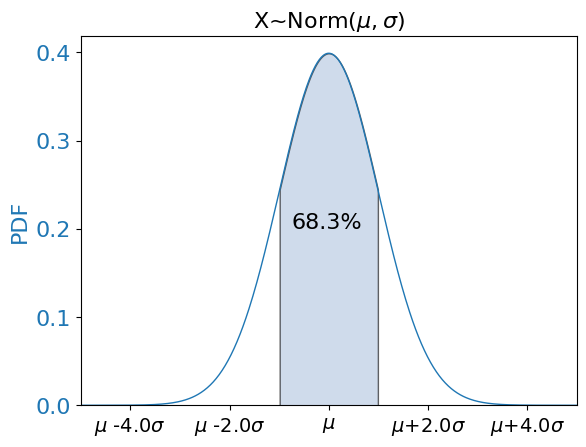
\includegraphics[scale=0.4]{Norm1sigma}

\end{column}
\end{columns}
\vspace{0.5cm}
\normalsize
\textcolor{magenta}{This term: $z=\frac{x-\mu}{\sigma}$ has many names: score, $z$-score, $z$-statistic, pull...}

\end{frame} 


% Norm, negative, quadratic
\begin{frame}{Features of the Gaussian \hfill \small{\bhl{$f_X(x;\mu,\sigma) = \textcolor<1>{red}{\frac{1}{\textcolor<5->{red}{\sigma} \sqrt{2\pi}}} e^{-\frac{1}{2} \frac{\textcolor<2>{red}{(x-\textcolor<3-4>{red}{\mu})}^2}{\textcolor<5->{red}{\sigma}^2}}$}}}
\small
\begin{columns}
\begin{column}{0.4\textwidth}
\begin{enumerate}
\item<1-> The normalisation coefficient is \textcolor<1>{red}{$\frac{1}{\sigma \sqrt{2\pi}} $}
\item<2-> The \textcolor<2>{red}{$x-\mu$} ensures symmetry around the mean, $\mu$.
\item<3-> \textbf{The location parameter is \textcolor<3-4>{red}{$\mu$}: shift left/right}\\
\item<5-> \textbf{The scale parameter is \textcolor<5->{red}{$\sigma$}: stretch/squish}\\
\end{enumerate}
\end{column}
\begin{column}{0.6\textwidth}

\only<1-2>{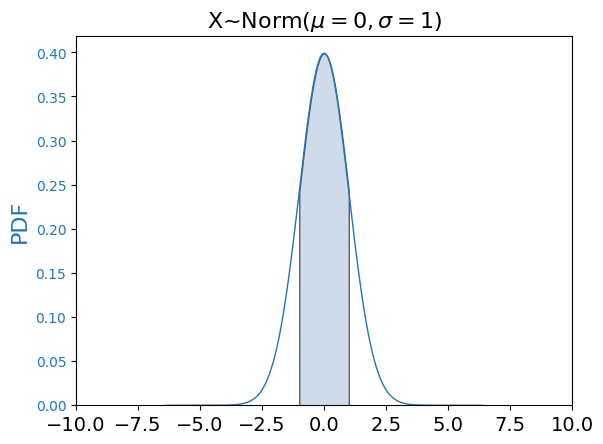
\includegraphics[scale=0.4]{Norm1sigma_mu0_sigma1.png}}
\only<3>{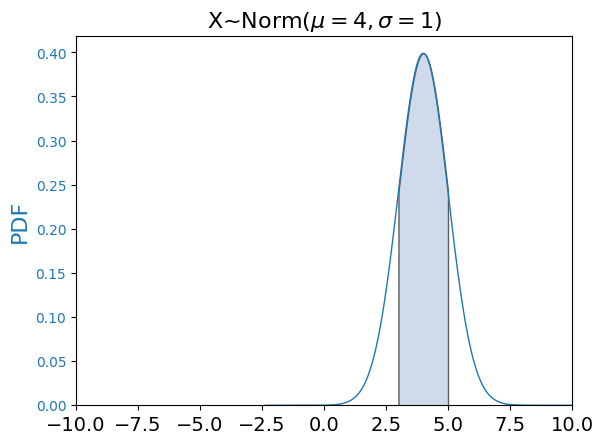
\includegraphics[scale=0.4]{Norm1sigma_mu4_sigma1.png}}
\only<4>{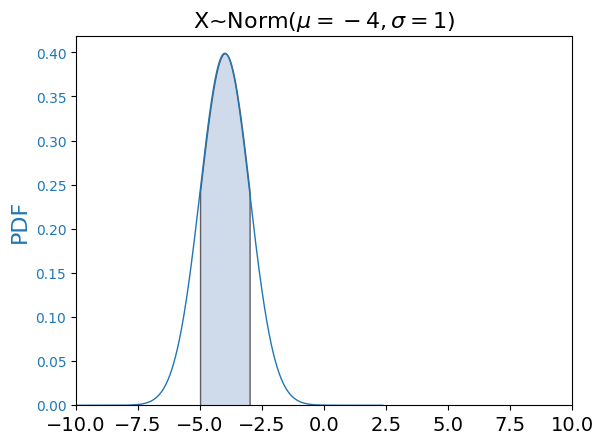
\includegraphics[scale=0.4]{Norm1sigma_mu-4_sigma1.png}}
\only<5>{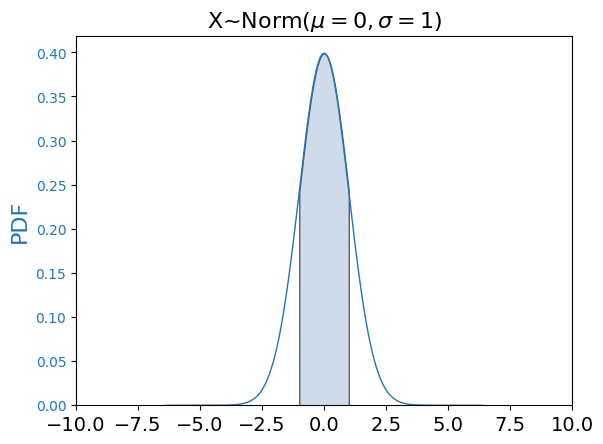
\includegraphics[scale=0.4]{Norm1sigma_mu0_sigma1.png}}
\only<6>{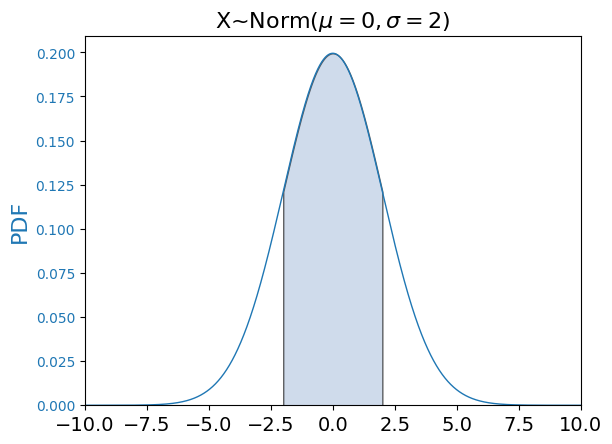
\includegraphics[scale=0.4]{Norm1sigma_mu0_sigma2.png}}
\only<7>{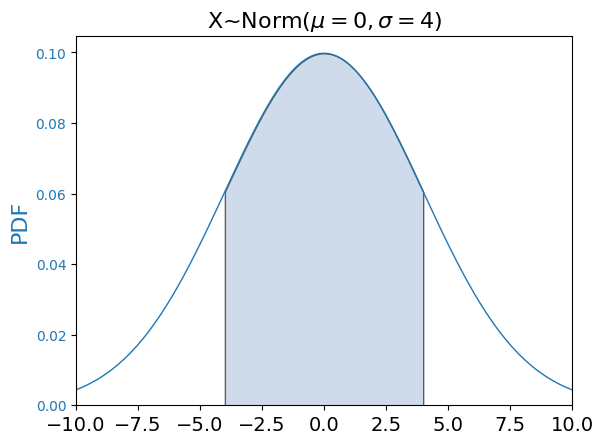
\includegraphics[scale=0.4]{Norm1sigma_mu0_sigma4.png}}

\end{column}
\end{columns}
\end{frame} 


% maximum, log
\begin{frame}{More features of the Gaussian \hfill \small{\bhl{$f_X(x;\mu,\sigma) = \frac{1}{\sigma \sqrt{2\pi}} e^{-\frac{1}{2} \frac{(x-\mu)^2}{\sigma^2}}$}}}
\small
\begin{columns}
\begin{column}{0.4\textwidth}
\begin{enumerate}
\item<1-> The maximum of the PDF is at $x=\mu$, because $e^{0}=1$
\item<1-> The maximum of the PDF is $\frac{1}{\sigma \sqrt{2\pi}}$
\item<2-> The (natural) log ($\ln$) of the PDF is quadratic in $x$.
\item<4-> Quadratic in $x$: bowl shaped
\item<4-> Negative quadratic: inverted bowl
\end{enumerate}
\end{column}
\begin{column}{0.6\textwidth}
\centering
\only<1>{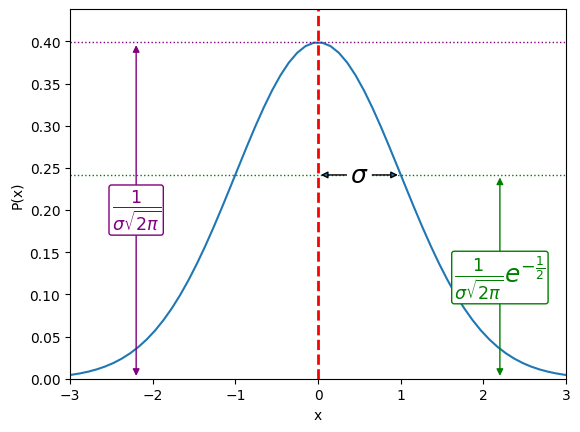
\includegraphics[scale=0.4]{PLOTDAT-MeanSigmaFWHM.png}}
\only<2>{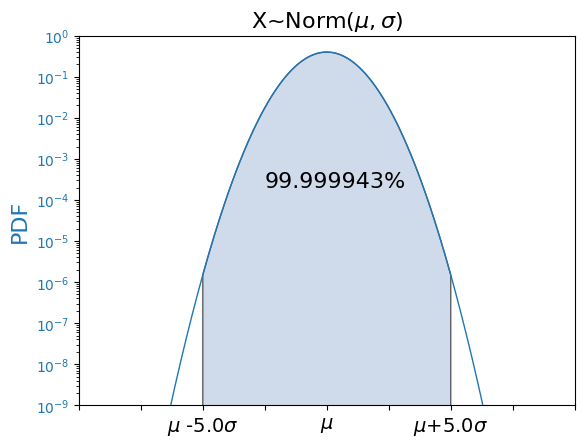
\includegraphics[scale=0.4]{Norm5sigmaLog}
\blu{semilogy(x,PDF)}
}
\only<3->{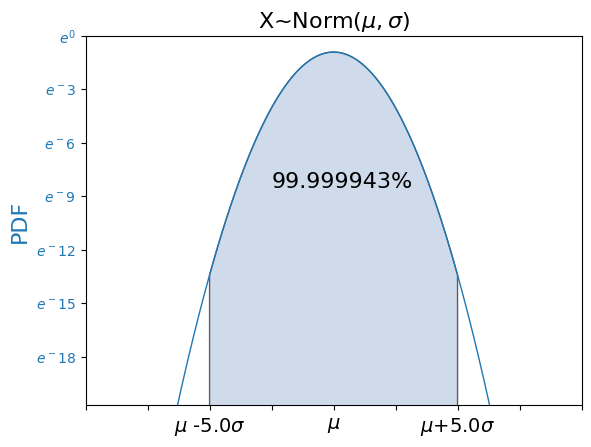
\includegraphics[scale=0.4]{Norm5sigmaLogNat}
\blu{semilogy(x,PDF, base=np.e)}
}
\end{column}
\end{columns}
\end{frame} 



\begin{frame}{Log of Gaussian PDF  \hfill \small{\bhl{$f_X(x;\mu,\sigma) = \frac{1}{\sigma \sqrt{2\pi}} e^{-\frac{1}{2} \frac{(x-\mu)^2}{\sigma^2}}$}}}
\small

\begin{align*}
\ln{f_X(x;\mu,\sigma)} &= \ln{ \left[ \frac{1}{\sigma \sqrt{2\pi}} e^{-\frac{1}{2} \frac{(x-\mu)^2}{\sigma^2} } \right] }&\\
\uncover<2->{ &= \ln{\left[ \dfrac{1}{\sigma \sqrt{2\pi}} \right]} + \ln{\left[ e^{-\frac{1}{2} \frac{(x-\mu)^2}{\sigma^2} } \right]}&\blu{\;because\; \ln{ab} = \ln{a} + \ln{b}}
}\\
\uncover<3->{              &= \ln{\left[ \dfrac{1}{\sigma \sqrt{2\pi}} \right]} -\frac{1}{2} \frac{(x-\mu)^2}{\sigma^2}  &\blu{\;because\; \ln{e^a} = a} }\\
\uncover<4->{              &= -\ln{ \sigma \sqrt{2\pi}} -\frac{1}{2} \frac{(x-\mu)^2}{\sigma^2} &\blu{\;because\; \ln{\frac{1}{a}} = -\ln{a} }}\\
\uncover<5->{              &= -\ln{ \sigma} -\ln{ \sqrt{2\pi} } - \frac{1}{2} \frac{(x-\mu)^2}{\sigma^2} &\blu{\;because\; -\ln{ab} = -\ln{a} - \ln{b}} } \\		
\end{align*}
\uncover<5->{\textcolor{magenta}{This will be useful to us when we come to maximising the log likelihood for parameter estimation.}}
\end{frame} 

\section{Multivariate Gaussian}



%============================%
% Univariate to Multivariate
%============================%
\begin{frame}{Gaussian: Univariate to Multivariate }
\large
\visible<1-2>{
Univariate: \\
$f_X(x;\mu,\sigma) = \dfrac{1}{\textcolor<2>{blue}{\sigma} \sqrt{2\pi}} \exp[-\dfrac{1}{2} \dfrac{(x-\mu)^2}{\sigma^2}]$\\[2ex]

Multivariate: \\
$f_X(x;\mu,\covmat) =\dfrac{ 1}{\textcolor<2>{blue}{ |\covmat|^{1/2}}  (2\pi)^{Z/2}} \exp\left[-\frac{1}{2} (x-\mu)^\mathsf{T} \covmat^{-1} (x-\mu) \right]$\\[2ex]
}

\only<1>{
\centering
Yikes.
}
\normalsize
\only<2>{

\textcolor{blue}{
In the normalisation we have $\sigma \rightarrow |\covmat|^{1/2}$}\\[1ex]
%This makes sense because $|\Sigma| = \prod\limits_j^Z \sigma_j^2$\\[1ex]
\purp{We also have $\sqrt{2\pi} \rightarrow (2\pi)^{Z/2}$ to keep the PDF valid ($Z$ is the number of RVs).}\\
}
%\only<3>{
%
%\textcolor{blue}{In place of the squared pull $\dfrac{(x-\mu)^2}{\sigma^2}$, we have the multivariate version: $(x-\mu)^\mathsf{T} \covmat^{-1} (x-\mu) $.\\[1ex]
%$\covmat^{-1}$ is the inverse of the covariance matrix.
%}
%}
\end{frame} 

%============================%
% Dealing with the normalisation 1. Determinant, 2. Norm
%============================%
\begin{frame}{Example: Two Independent RVs \textcolor{blue}{\only<1>{[1. Determinant]} \only<2>{[2. Normalisation]}}}

$
x = \begin{bmatrix}
x_1\\
x_2
 \end{bmatrix}\;\;
 \mu = \begin{bmatrix}
\mu_1\\
\mu_2
 \end{bmatrix} \;\; 
 \covmat = \begin{bmatrix}
\sigma^2_1 & 0\\
0 & \sigma^2_2 \\
 \end{bmatrix} 
$
 \textcolor{magenta}{$\leftarrow$ Independent RVs: $\covmat$ diagonal.}

\vspace{0.5cm}

$f_X(x;\mu,\covmat)  =\textcolor<2>{blue}{\dfrac{ 1}{\textcolor<1>{blue}{ |\covmat|^{1/2}}  (2\pi)^{Z/2}} }\exp[-\frac{1}{2} 
(x-\mu)^\mathsf{T} \covmat^{-1} (x-\mu)
]
$\\
\vspace{0.5cm}

\only<1-2>{
\textcolor<1>{blue}{
$|\covmat|^{1/2}  = \begin{vmatrix}
\sigma^2_1 & 0\\
0 & \sigma^2_2 \\
 \end{vmatrix}^{1/2}  = ( \sigma^2_1 \sigma^2_2 - 0 0 )^{1/2} = \sigma_1 \sigma_2$}\\
\vspace{0.5cm}

\uncover<2>{
\textcolor{blue}{
$\dfrac{ 1}{|\covmat|^{1/2}  (2\pi)^{Z/2}}  = \dfrac{1}{ \sigma_1 \sigma_2 2\pi}$}\\
}}
\end{frame} 



%============================%
% Dealing with the argument
%============================%
\begin{frame}{Example: Two Independent RVs \textcolor{magenta}{
\only<1-2>{[3. Cov Matrix]} 
\only<3>{[4. Multiply]}
\only<4>{[5. Multiply]}
}
}

$
x = \begin{bmatrix}
x_1\\
x_2
 \end{bmatrix}\;\;
 \mu = \begin{bmatrix}
\mu_1\\
\mu_2
 \end{bmatrix} \;\; 
 \covmat = \begin{bmatrix}
\sigma^2_1 & 0\\
0 & \sigma^2_2 \\
 \end{bmatrix} 
$
\vspace{0.5cm}

$f_X(x;\mu,\covmat)  =\textcolor{blue}{\dfrac{1}{ \sigma_1 \sigma_2 2\pi}}\exp[-\frac{1}{2} 
\textcolor<4>{magenta}{(x-\mu)^\mathsf{T}} \textcolor<1-4>{magenta}{\covmat^{-1}}\textcolor<3-4>{magenta}{ (x-\mu)}
]
$\\
\vspace{0.5cm}


% SLIDE 2: INVERSE OF COV MATRIX
\only<2>{
\textcolor<2>{magenta}{
$
\begin{bmatrix}
\sigma^2_1 & 0\\
0 & \sigma^2_2 \\
 \end{bmatrix}^{-1}  =
\begin{bmatrix}
\frac{1}{\sigma^2_1} & 0\\
0 & \frac{1}{\sigma^2_2} \\
 \end{bmatrix} 
 $
 }
 \\[2ex]
 \magt{Warning! We can only invert a matrix like this if it is diagonal!} Finding the inverse of a matrix is usually a total faff.
 }
 
 % SLIDE 3: INVERSE OF COV MATRIX TIMES X-MU
\only<3>{
\textcolor<3>{magenta}{
$
\begin{bmatrix}
\frac{1}{\sigma^2_1} & 0\\
0 & \frac{1}{\sigma^2_2} \\
 \end{bmatrix} \begin{bmatrix}
x_1 - \mu_1\\
x_2 -\mu_2
 \end{bmatrix}
 =
 \begin{bmatrix}
\frac{1}{\sigma^2_1} (x_1 - \mu_1)\\
\frac{1}{\sigma^2_2}  (x_2 - \mu_2)\\
 \end{bmatrix} 
 $
 }
 \\[2ex]
 }
 
  % SLIDE 4: INVERSE OF COV MATRIX TIMES X-MU and TRANS
\only<4>{
\textcolor<4>{magenta}{
$
\begin{bmatrix}
x_1 - \mu_1\\
x_2 -\mu_2
 \end{bmatrix}^{\mathsf{T}}
 \begin{bmatrix}
\frac{1}{\sigma^2_1} (x_1 - \mu_1)\\
\frac{1}{\sigma^2_2}  (x_2 - \mu_2)\\
 \end{bmatrix} 
 =
 \dfrac{ (x_1 - \mu_1)^2 }{\sigma^2_1} +  \dfrac{ (x_2 - \mu_2)^2}{\sigma^2_2} 
 $
 }
 \\[2ex]
 }
 \end{frame} 



%============================%
% EXP TERM IN FULL
%============================%
\begin{frame}{Example: $Z=2$ independent RVs \textcolor{darkgreen}{
\only<1->{[6. Full Argument]}
}}

$
x = \begin{bmatrix}
x_1\\
x_2
 \end{bmatrix}\;\;
 \mu = \begin{bmatrix}
\mu_1\\
\mu_2
 \end{bmatrix} \;\; 
 \Sigma = \begin{bmatrix}
\sigma^2_1 & 0\\
0 & \sigma^2_2 \\
 \end{bmatrix} 
$
\vspace{0.5cm}

$f_X(x;\mu,\Sigma)  =\textcolor{blue}{\dfrac{1}{ \sigma_1 \sigma_2 2\pi}}
\textcolor<2>{darkgreen}{\exp[-\dfrac{1}{2} \left[
\textcolor<1>{magenta}{
 \dfrac{ (x_1 - \mu_1)^2 }{\sigma^2_1} +  \dfrac{ (x_2 - \mu_2)^2}{\sigma^2_2} 
}
\right]
]}
$\\
\vspace{0.5cm}

\only<2>{
\textcolor<2>{darkgreen}{
$
%\exp[- \frac{1}{2\sigma^2_1}  (x_1 - \mu_1)^2 -  \frac{1}{2\sigma^2_2}  (x_2 - \mu_2)^2]
%=
e^{- A -  B}
=
e^{- A}e^{ -B}
%\exp[-\frac{1}{2\sigma^2_1}  (x_1 - \mu_1)^2] \exp[-\frac{1}{2\sigma^2_2}  (x_2 - \mu_2)^2]
%=
%e^{-\frac{1}{2}\dfrac{(x_1 - \mu_1)^2}{\sigma^2_1}} e^{-\dfrac{1}{2\sigma^2_2}  (x_2 - \mu_2)^2}
 $
 }
 \\[2ex]

$f_X(x;\mu,\Sigma)  =
\textcolor{blue}{\dfrac{1}{ \sigma_1 \sigma_2 2\pi}}
\textcolor<2>{darkgreen}{\exp[-\dfrac{(x_1 - \mu_1)^2}{2\sigma^2_1}]\, \exp[-\dfrac{(x_2 - \mu_2)^2}{2\sigma^2_2}  ]}
$\\
 }
 
 \end{frame}
 
 
 
 %============================%
% RESULT
%============================%
\begin{frame}{Example: $Z=2$ independent RVs \textcolor{darkgreen}{
\only<1->{[7. Result]}
}}
$
x = \begin{bmatrix}
x_1\\
x_2
 \end{bmatrix}\;\;
 \mu = \begin{bmatrix}
\mu_1\\
\mu_2
 \end{bmatrix} \;\; 
 \covmat = \begin{bmatrix}
\sigma^2_1 & 0\\
0 & \sigma^2_2 \\
 \end{bmatrix} 
$
\vspace{1cm}

\only<1>{
$f_X(x;\mu,\covmat)  =
\textcolor{blue}{\dfrac{1}{ \sigma_1 \sigma_2 2\pi}} \textcolor{darkgreen}{\exp[-\dfrac{(x_1 - \mu_1)^2}{2\sigma^2_1}]\, \exp[-\dfrac{(x_2 - \mu_2)^2}{2\sigma^2_2}  ]}$
}
\only<2>{
$f_X(x;\mu,\covmat)  =
\textcolor{blue}{\dfrac{1}{ \sigma_1  \sqrt{2\pi}}}\textcolor{darkgreen}{\exp[-\dfrac{(x_1 - \mu_1)^2}{2\sigma^2_1}]}\,\textcolor{blue}{\dfrac{1}{ \sigma_2  \sqrt{2\pi}}} \textcolor{darkgreen}{\exp[-\dfrac{(x_2 - \mu_2)^2}{2\sigma^2_2}  ]}$

\vspace{0.5cm}

\bbl{A multivariate Gaussian PDF with two independent RVS is the product of the Gaussian PDF for each of the RVs.}\\[1ex]

$ f_X(x;\mu,\covmat) = f_X(x_1;\mu_1,\sigma_1)\, f_X(x_2;\mu_2,\sigma_2) $
}
 \end{frame}


 %============================%
% Isocontours
%============================%


\begin{frame}{Bivariate Gaussian Visually: Error Ellipses}
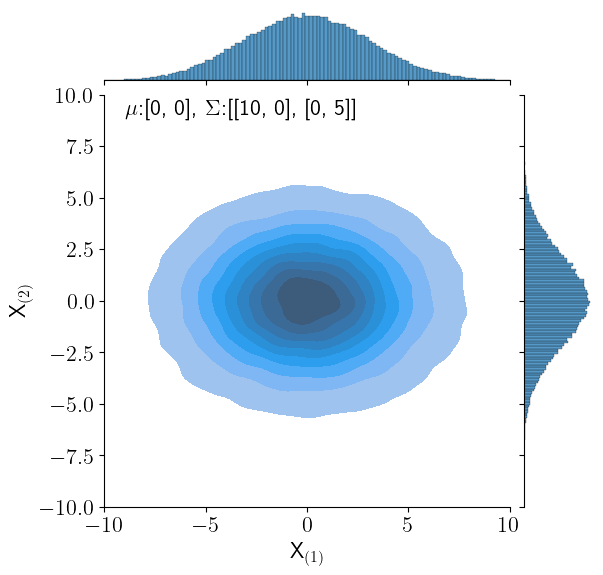
\includegraphics[scale=0.32]{BivariateGaussian-mu-0-0-cov-10-0-0-5.png}
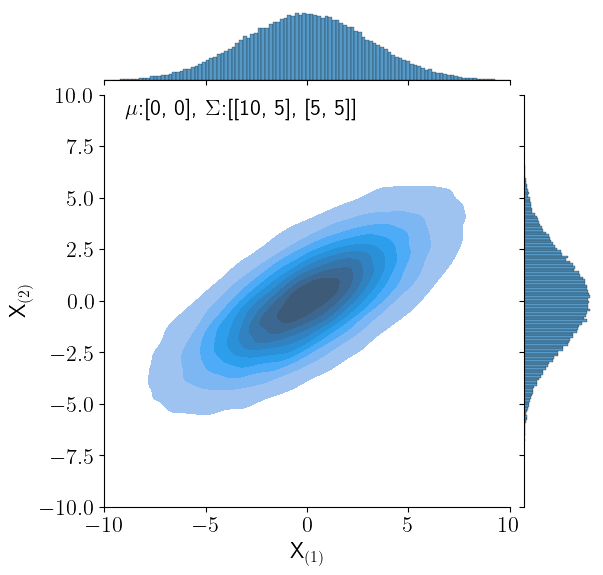
\includegraphics[scale=0.32]{BivariateGaussian-mu-0-0-cov-10-5-5-5.png}

\footnotesize
On these plots the value of the PDF is mapped to colour. \boo{Isocontours} have the same colour: same probability.\\
\end{frame}

\begin{frame}{Bivariate Gaussian: Error Ellipses}
\footnotesize
\boo{Isocontours} have  constant  probability $f_X(x;\mu,\Sigma)= c$\\

$c = 
\dfrac{1}{ \sigma_1 \sigma_2 2\pi}
\exp[-\left[
 \dfrac{ (x_1 - \mu_1)^2 }{2\sigma^2_1} +  \dfrac{ (x_2 - \mu_2)^2}{2\sigma^2_2} 
\right]
]  $ \;\;\; \blu{Joint probability=constant} \\[1ex]

\uncover<2->{
$\ln{( \sigma_1 \sigma_2 2\pi c)} = 
-\left[
 \dfrac{ (x_1 - \mu_1)^2 }{2\sigma^2_1} +  \dfrac{ (x_2 - \mu_2)^2}{2\sigma^2_2} 
\right]  $\;\;\;\;\;\; \blu{Log of both sides} \\[1ex]
}
\uncover<3->{
$\ln{\dfrac{1}{( \sigma_1 \sigma_2 2\pi c)}} = 
 \dfrac{ (x_1 - \mu_1)^2 }{2\sigma^2_1} +  \dfrac{ (x_2 - \mu_2)^2}{2\sigma^2_2} 
 $\;\;\;\;\;\; \blu{$-\ln(a) = \ln \dfrac{1}{a}$} \\[1ex]
}
\uncover<4->{
$1 = 
 \dfrac{ (x_1 - \mu_1)^2 }{\textcolor{blue}{2\sigma^2_1 (\ln{\frac{1}{( \sigma_1 \sigma_2 2\pi c)}})}} +
 \dfrac{ (x_2 - \mu_2)^2 }{\textcolor{red}{2\sigma^2_2 (\ln{\frac{1}{( \sigma_1 \sigma_2 2\pi c)}})}} 
 $
 }
 \uncover<5->{
 \bhl{$= 
 \dfrac{ (x_1 - \mu_1)^2 }{\textcolor{blue}{r^2_1}} +
 \dfrac{ (x_2 - \mu_2)^2 }{\textcolor{red}{r^2_2}} 
 $}
 }
  \\[1ex]
 
  \uncover<5->{
 This is the equation of an ellipse with semi-major axis \textcolor{blue}{$r_1$} and semi-minor axis \textcolor{blue}{$r_2$}\\[1ex]
 }
 
\end{frame}

\begin{frame}{Ellipse}

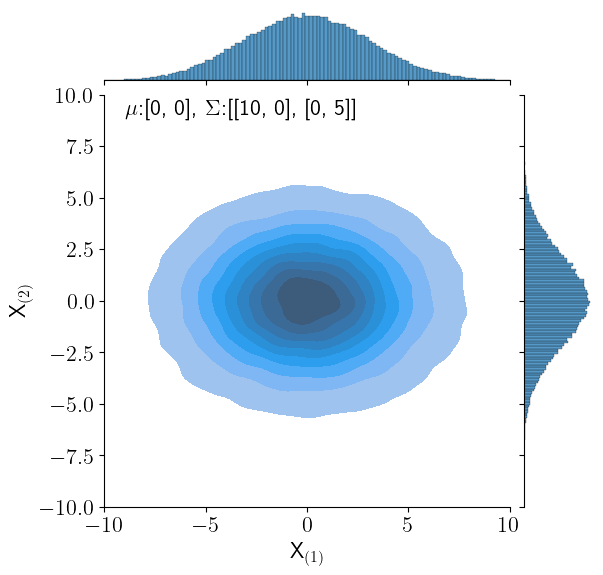
\includegraphics[scale=0.32]{BivariateGaussian-mu-0-0-cov-10-0-0-5.png}
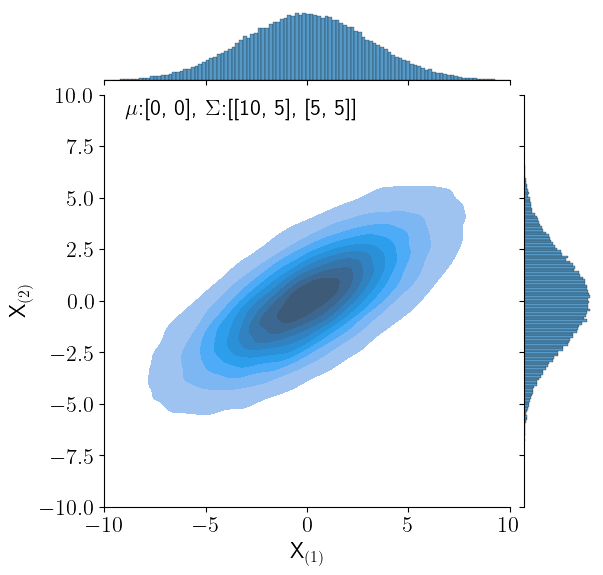
\includegraphics[scale=0.32]{BivariateGaussian-mu-0-0-cov-10-5-5-5.png}

\end{frame}



\begin{frame}{Principal Components}
\footnotesize

$1 = 
 \dfrac{ (x_1 - \mu_1)^2 }{\textcolor{blue}{2\sigma^2_1 (\ln{\frac{1}{( \sigma_1 \sigma_2 2\pi c)}})}} +
 \dfrac{ (x_2 - \mu_2)^2 }{\textcolor{red}{2\sigma^2_2 (\ln{\frac{1}{( \sigma_1 \sigma_2 2\pi c)}})}} 
 = 
 \dfrac{ (x_1 - \mu_1)^2 }{\textcolor{blue}{r^2_1}} +
 \dfrac{ (x_2 - \mu_2)^2 }{\textcolor{red}{r^2_2}} 
 $ \\[1ex]
 
 This is the equation of an ellipse with \textcolor{magenta}{semi-major axis} \textcolor{blue}{$r_1$} and \textcolor{magenta}{semi-minor axis} \textcolor{red}{$r_2$}\\[1ex]
 
 This is cool because the height of the Gaussian at $1\sigma$ half-width is $c_{1\sigma} =\dfrac{1}{e \sigma_1 \sigma_2 2\pi}$ and if we plug this into our ellipse radii we get the \gbl{simple form}:\\[1ex]
 
$ r_j =\sqrt{2\sigma^2_j (\ln{\frac{1}{ \sigma_1 \sigma_j 2\pi (\frac{1}{e \sigma_1 \sigma_2 2\pi} ) } ) } } = 
\gbl{\sqrt{ 2}\sigma_j}$\\[1ex]

\textcolor{magenta}{The $r_j$ are the Principal Components} of the data. In this example there are only two dimensions, but we have rotated them such that they are in the directions of maximum variance.

\end{frame}

\begin{frame}{Principal Components}
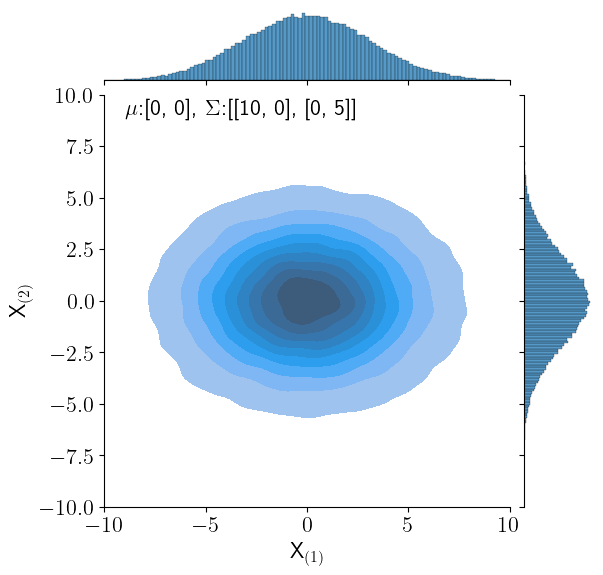
\includegraphics[scale=0.32]{BivariateGaussian-mu-0-0-cov-10-0-0-5.png}
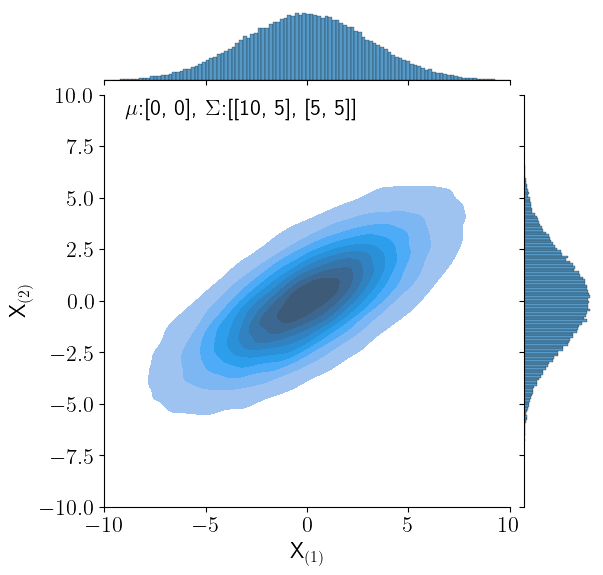
\includegraphics[scale=0.32]{BivariateGaussian-mu-0-0-cov-10-5-5-5.png}
\footnotesize

% This is cool because the height of the Gaussian at $1\sigma$ half-width is $c_{1\sigma} =\dfrac{1}{e \sigma_1 \sigma_2 2\pi}$ and if we plug this into our ellipse radii we get the simple form:\\[1ex]
 
%$ r_j =\sqrt{2\sigma^2_j (\ln{\frac{1}{ \sigma_1 \sigma_j 2\pi (\frac{1}{\sigma_1 \sigma_2 2\pi} ) } ) } } = \sqrt{ 2}\sigma_j$\\[1ex]

\textcolor{magenta}{Principal Component Analysis is useful when we have high dimensional data and want to reduce it to two dimensions: the two with maximum variance. Nice intro \href{https://builtin.com/data-science/step-step-explanation-principal-component-analysis}{here}.}
\end{frame}


%https://medium.com/data-science/unraveling-the-law-of-large-numbers-e36a3219acb2

\section{LLN}

\begin{frame}{The Law(s) of Large Numbers}
\small

The \magtn{Weak Law of Large Numbers} (LLN):\\
\begin{center}
\ghl{$\lim\limits_{N\to \infty} P(| \overline{x} - \mu | \geq \alpha) =0\; \mathsf{for}\; \alpha > 0 $}\\[1ex]
\end{center}
The Weak LLN states that there is a high probability that the sample mean $\overline{x}$ will approach the expected value (true mean $E[X] \equiv \mu$)  in the limit of an infinite number of measurements. \\

The Strong LLN: $P(\lim\limits_{N\to \infty} \overline{x} = \mu) =1$.\\

The difference between these is fairly subtle, with the Strong LLN indicating \textbf{almost sure} convergence (almost sure is a statistical term).\\

\end{frame}


\begin{frame}{The Weak LLN \hfill \small{\ghl{$\lim\limits_{N\to \infty} P(| \overline{x} - \mu | \geq \textcolor{blue}{\alpha}) =0\; \mathsf{for}\; \alpha > 0 $}}}
\footnotesize
%$\lim\limits_{N\to \infty} P(| \overline{x} - \mu | \geq \textcolor{blue}{\alpha}) =0\; \mathsf{for}\; \alpha > 0 $\\

\only<1>{
We have referred to the Weak LLN previously when we looked at how the mean \textbf{tends to approach} the expected value as we increase $N$:\\[1ex]

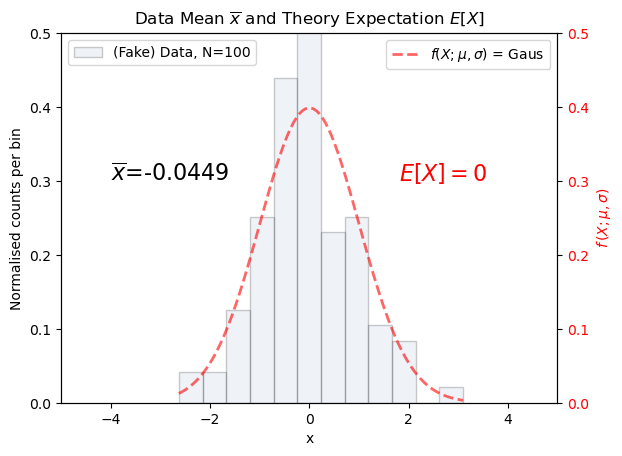
\includegraphics[scale=0.3]{PLOTDAT2-MeanAndExpec_Norm_Mu0_Sigma1_N100.png}
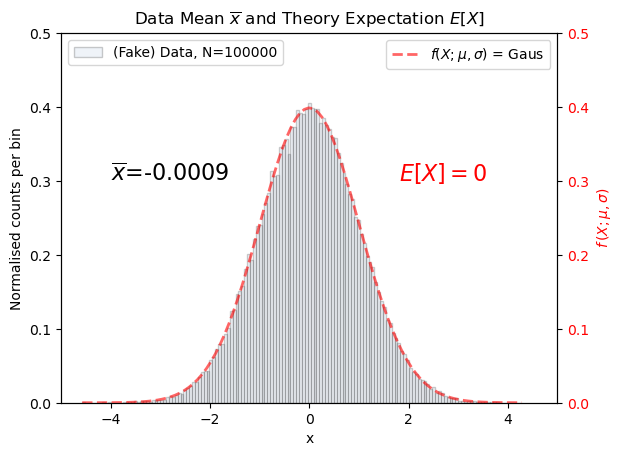
\includegraphics[scale=0.3]{PLOTDAT2-MeanAndExpec_Norm_Mu0_Sigma1_N100000.png}
}
\only<2>{
\begin{columns}
\begin{column}{0.5\textwidth}
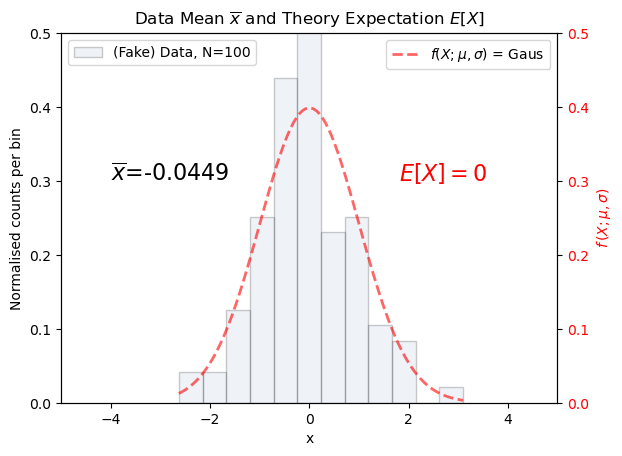
\includegraphics[scale=0.35]{PLOTDAT2-MeanAndExpec_Norm_Mu0_Sigma1_N100.png} 
\end{column}
\begin{column}{0.5\textwidth}
\small
\textcolor{magenta}{$\leftarrow$ For this \textbf{single experiment}}\\[1ex]
$| \overline{x} - \mu | =0.0449= \alpha_1$
\end{column}
\end{columns}
}
\only<3>{
\begin{columns}
\begin{column}{0.5\textwidth}
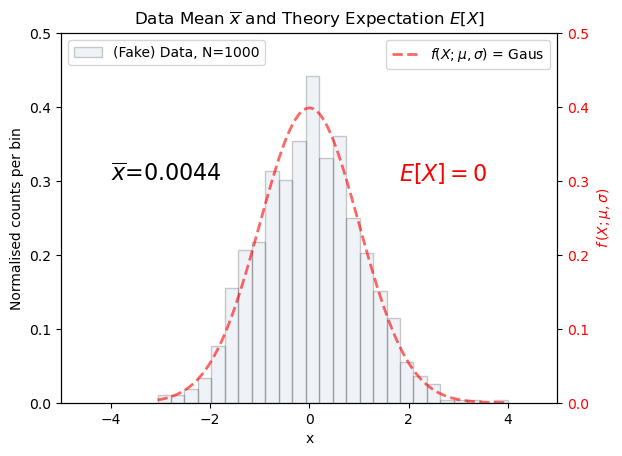
\includegraphics[scale=0.35]{PLOTDAT2-MeanAndExpec_Norm_Mu0_Sigma1_N1000.png} 
\end{column}
\begin{column}{0.5\textwidth}
\small
\textcolor{magenta}{$\leftarrow$ For this \textbf{single experiment}}\\[1ex]
$| \overline{x} - \mu | =0.0044= \alpha_1$
\end{column}
\end{columns}
}
\only<4>{
\begin{columns}
\begin{column}{0.5\textwidth}
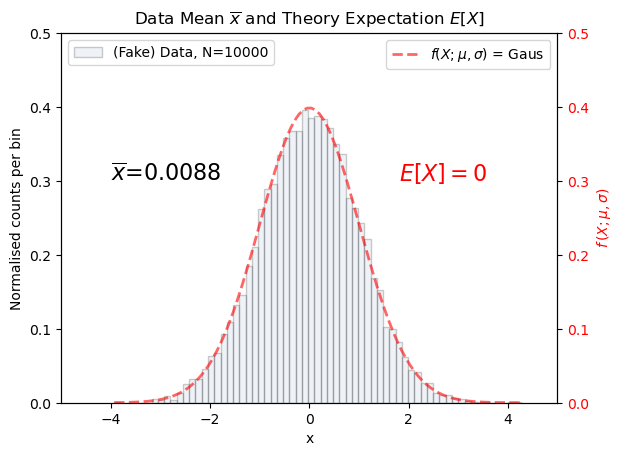
\includegraphics[scale=0.35]{PLOTDAT2-MeanAndExpec_Norm_Mu0_Sigma1_N10000.png} 
\end{column}
\begin{column}{0.5\textwidth}
\small
\textcolor{magenta}{$\leftarrow$ For this \textbf{single experiment}}\\[1ex]
$| \overline{x} - \mu | =0.0088= \alpha_1$
\end{column}
\end{columns}
}

\only<1>{The $N=100$ experiment has $| \overline{x} - \mu | =0.0449= \alpha_1$. If we have chosen a \textcolor{blue}{tolerance} of \textcolor{blue}{$\alpha=0.1$}, then $\alpha_1 < \textcolor{blue}{\alpha}$: a successful outcome. If we have chosen a \textcolor{blue}{tolerance} of \textcolor{blue}{$\alpha=10^{-9}$}, then $\alpha_1 > \textcolor{blue}{\alpha}$: this is a failure.}
\only<2> {If we were to repeat the $N=100$ experiment in the plot a thousand times ($Z\mathord{=}1k$), we would have a thousand $\alpha_j$ values. Some fraction of these will fall within our \textcolor{blue}{tolerance}. \\
\textcolor{magenta}{The plot above yields a single $\alpha_j=\alpha_1$: it is just one of our one thousand experiments. }}
\only<3>{If we increase $N=1000$, and keep $Z\mathord{=}1k$, we will find that a larger fraction of $\alpha_j$ fall within our \textcolor{blue}{tolerance}. \\
\textcolor{magenta}{Again, the plot above yields a single $\alpha_j$: it is just one of our $Z\mathord{=}1k$ experiments. }}
\only<4>{If we increase $N=10,000$, we will find that an even larger \textbf{fraction} of $\alpha_j$ fall within our \textcolor{blue}{tolerance}. \\
\textcolor{magenta}{The $\alpha_1$ for this single experiment has increased! That's okay, it is just one of our $Z\mathord{=}1k$ experiments. }}
\end{frame}

\begin{frame}{The Weak LLN \hfill \small{\ghl{$\lim\limits_{N\to \infty} P(| \overline{x} - \mu | \geq \textcolor{blue}{\alpha}) =0\; \mathsf{for}\; \alpha > 0 $}}}
\footnotesize


In the limit where our sample size $N$ approaches $\infty$, the fraction of means falling outside our tolerance approaches zero. This is true for any non-zero value of tolerance, $\alpha$.\\[1ex]

This is a \textbf{Probability Limit}. Can also be written:  $\plim\limits_{N\to \infty}  \overline{x} =\mu$\\[1ex]

\boo{This does not mean that the sample mean approaches the population mean as the sample size grows}. We have seen that is not necessarily the case.\\[1ex]

The Weak LLN tells us that the probability converges. It does not tell us that the value of the sample mean converges.\\

The Weak LLN only applies to the mean, not to the variance or other statistics.\\[1ex]

\end{frame}

\begin{frame}{Bernoulli's Weak LLN \hfill \small{\ghl{$\lim\limits_{N\to \infty} P(| \bbl{\overline{x} - \mu} | \geq \alpha) =0\; \mathsf{for}\; \alpha > 0 $}}}
\footnotesize

Bernoulli's LLN:\\[1ex]

$\lim\limits_{N\to \infty} P\left(\bigg| \bbl{\dfrac{k}{n} - p} \bigg| \geq \alpha\right) =0\; \;\mathsf{for}\; \alpha > 0$\\[1ex]

Here $\dfrac{k}{n}$ is the (measured) frequency of success and p is the (theoretical) probability of a successful outcome. \\

Recall that a Bernoulli trial repeated $n$ times is Binomial. The RV is $K$ and its expected value is $np$. So this is not any different from the regular weak LLN.\\[1ex]

This form is particularly useful for comparing histograms of data with PDFs, as the number of entries in a density histogram bin is a frequency for a range of the RV, and the area under the PDF is a probability for a range of the RV.

\end{frame}

\section{CLT}

\begin{frame}{Expected Value of the mean (`Mean of means') }
\footnotesize
In real life we will not have infinite datasets, but finite samples. We will calculate the sample mean $\overline{x}$. The Expected Value of the sample mean  is the population mean.
\begin{align*}
E\left[\, \overline{x}\, \right]  & = E\left[ \dfrac{1}{N} \sum\limits_i^N x_i \right] \blu{\; because\; \overline{x}  = \frac{1}{N} \sum \limits_i^N x_i}\\ 
 \uncover<2->{   & = \dfrac{1}{N} \sum\limits_i^N E\left[ x_i \right] \blu{\;because\; E[sum] = sum(E)} }\\
 \uncover<3->{   & = \dfrac{1}{N} \sum\limits_i^N E[X] \blu{\;because\; x_i\;are\; iid\; so\; E[x_i] = E[X]\; for\; all\; x_i}}\\
 \uncover<4->{   & = \dfrac{1}{N} N E[X]= E[X] }\\                                                
\end{align*}
 \uncover<4->{ The expected value of the sample mean of the independent, identically distributed (iid) measurements $x_i$ is the population (true) mean. Or, \textcolor{magenta}{the mean of the sample means is the population (true) mean.}}
\end{frame}

\begin{frame}{Variance on the mean}
\footnotesize


\begin{align*}
V\left[\, \overline{x}\, \right]  & = V\left[ \dfrac{1}{N} \sum\limits_i^N x_i \right] \blu{\; because\; \overline{x}  = \frac{1}{N} \sum \limits_i^N x_i}\\ 
 \uncover<2->{   &= \sum\limits_i^N  V\left[ \dfrac{1}{N}  x_i \right] \blu{\;because\; V[sum] = sum(V)\; for\; iid\; x_i}}\\
 \uncover<3->{   & = \dfrac{1}{N^2}  \sum\limits_i^N V\left[ x_i \right] \blu{\;because\;V\left[ax\right] = a^2 V\left[x\right] }}\\
 \uncover<4->{   & = \dfrac{1}{N^2} N V[X]  \blu{\;because\;V[X] = \frac{1}{N} \sum\limits_i^N (x_i-\overline{x})^2 
                          = \frac{1}{N} \sum\limits_i^N V[x_i]   }}\\
 \uncover<5->{   & = \dfrac{1}{N} V[X] }\\                                               
\end{align*}
 \uncover<5->{ The variance of the sample mean of the iid measurements is $\dfrac{1}{N}$ times the population (true) variance, $V[X]$.} \\[1ex]

\end{frame}


\begin{frame}{Variance on the mean (SEM: $\sigma_{\overline{x}}$) }
\footnotesize
\begin{center}
\ghl{$V\left[\, \overline{x}\, \right]  = \dfrac{1}{N} V[X] $}\\
\end{center}
\magtn{This is an important result} because it tells us that the uncertainty on the sample mean, $\sigma_{\overline{x}}$, goes like $\dfrac{1}{\sqrt{N}}$, where $N$ is the number of measurements.\\
\begin{center}
\ghl{$\sigma_{\overline{x}}  = \dfrac{1}{\sqrt{N}} \sigma_{true}$}
\end{center}
$\sigma_{\overline{x}}$ is known as the \magtn{Standard Error on the Mean} (SEM).\\

\begin{itemize}
\item $\sigma_{true}$ is irreducible: it is the true spread of values of a RV, because the RV is R:Random!
\item The measurement uncertainty $\sigma_{\overline{x}} $ will become smaller as we take more data, and has the true spread of the RV as a constant factor.
\end{itemize}
\end{frame}



\begin{frame}{The Central Limit Theorem}
\small

The Central Limit Theorem (CLT) states that the \magt{distribution of sample means $\overline{x}$} from any underlying PDF converges to a Gaussian distribution with mean $\mu$ and variance $\sigma^2/N$, as $N$ approaches infinity. The $N$ here is the number of measurements used to calculate the means.\\[1ex]

The mean is a normalised sum of $N$ measurements, so the CLT equivalently states that the  \magt{distribution of the sum of $N$ RVs} converges to Gaussian.\\[1ex]

\bbl{The means/RVs do not have to come from the Gaussian PDF - they can come from any PDF.} If you calculate $N\to\infty$ means (or sums) of RVs from a uniform, binomial, exponential \bbl{or any finite variance PDF}, the means will be normally distributed.\\[1ex]
\end{frame}

\begin{frame}{The Central Limit Theorem, Visually}
\footnotesize
\only<1>{
%It does not matter if you use the mean score or the sum score, the distributions are identical other than a scale factor (the values on the x-axis are scaled by $N$ for the sum, and the values on the y-axis are scaled down to ensure this is a density.)\\
\bbl{N=1}: I am calculating the mean (sum) of a single measurement (or a single RV). \magt{(Yes, this is silly, because the mean of one value is just the value!)} To fill the histogram, I have repeated the 1-measurement experiment $Z$ times.\\
}
\only<2>{
\bbl{N=2}: I am calculating the mean (sum) of two measurements (or, two RVs). \\
}
\only<3>{
\bbl{N=3}: I am calculating the mean (sum) of three measurements (or, three RVs). \\
}
\only<4->{
And so on.\\
}

\begin{center}
\only<1>{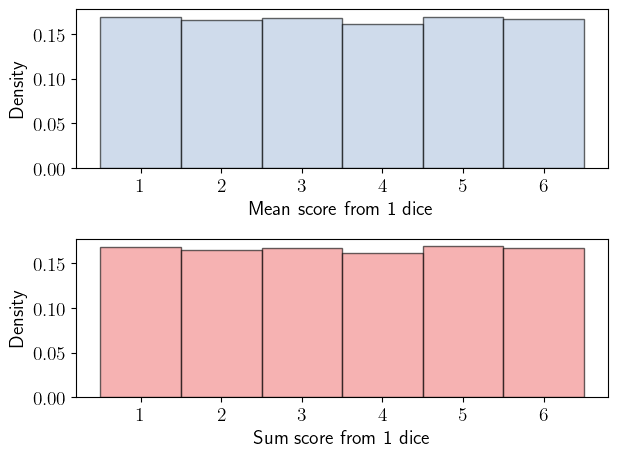
\includegraphics[scale=0.4]{CLT-uniform-N1-Z10000-meanandsum.png}}
\only<2>{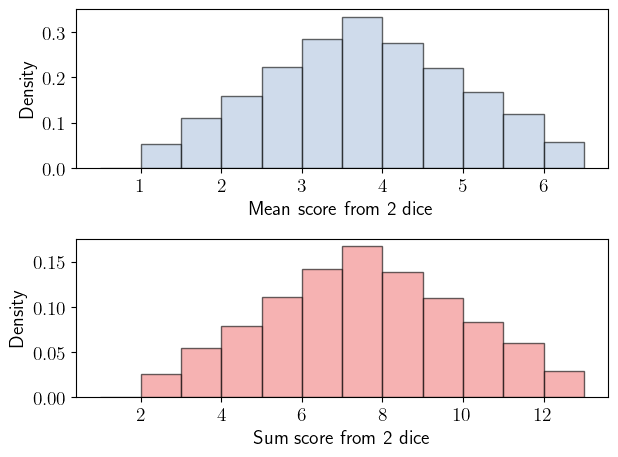
\includegraphics[scale=0.4]{CLT-uniform-N2-Z10000-meanandsum.png}}
\only<3>{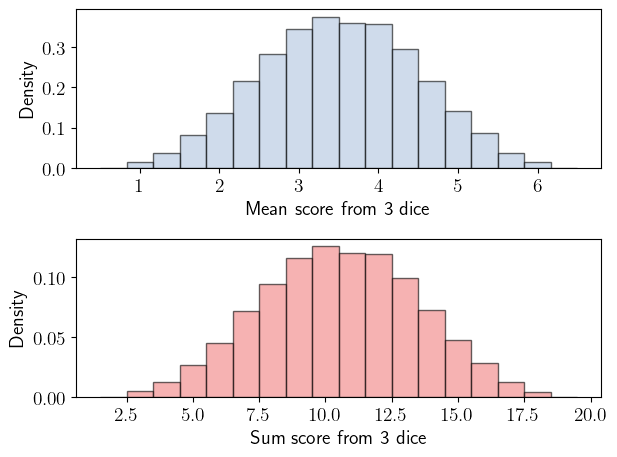
\includegraphics[scale=0.4]{CLT-uniform-N3-Z10000-meanandsum.png}}
\only<4>{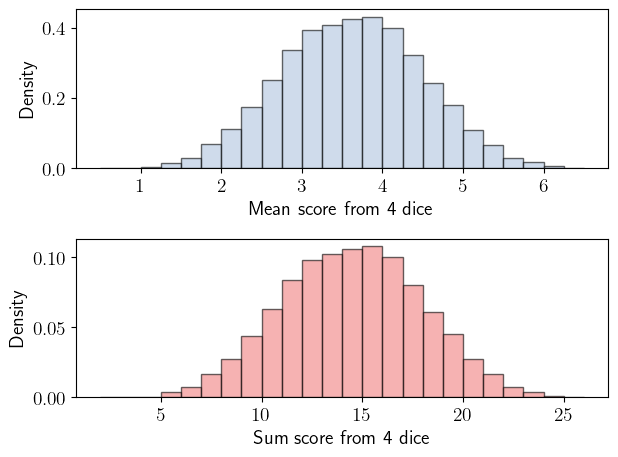
\includegraphics[scale=0.4]{CLT-uniform-N4-Z10000-meanandsum.png}}
\only<5>{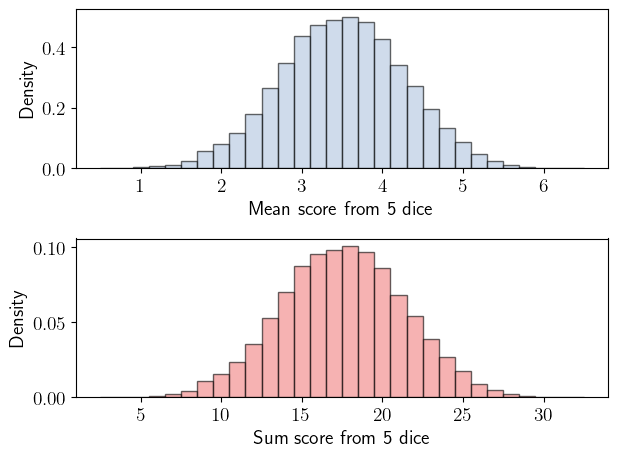
\includegraphics[scale=0.4]{CLT-uniform-N5-Z10000-meanandsum.png}}
\only<6>{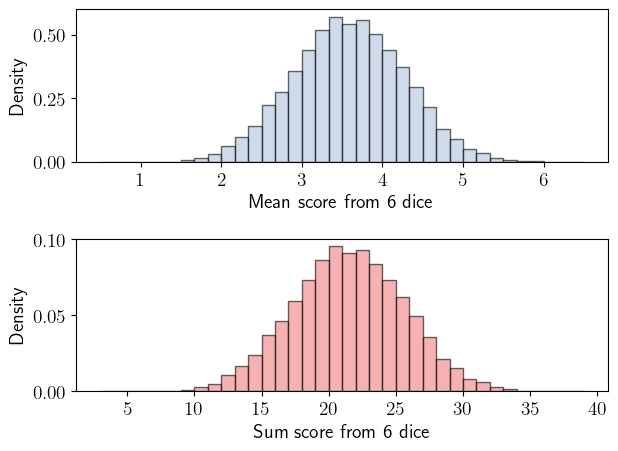
\includegraphics[scale=0.4]{CLT-uniform-N6-Z10000-meanandsum.png}}
 \end{center}
 \end{frame}
 
 \begin{frame}{The Central Limit Theorem, Visually}
\footnotesize

\only<1-4>{
As the number of RVs grows, we start to see the means (or sums) taking on a bell-shaped distribution. As $N\rightarrow\infty$ the distribution $\rightarrow$ Norm($\overline{x},\sigma_{samp}$).
}

\only<5>{
The distribution \textbf{of means} will approach a normal distribution in the limit $N\to\infty$, but in practice the distribution starts looking Gaussian much earlier.\\
The \boo{Central Limit} is the true mean $E[X] \equiv \mu$, which is quite stable as we increase $N$.
}

\begin{center}
\only<1>{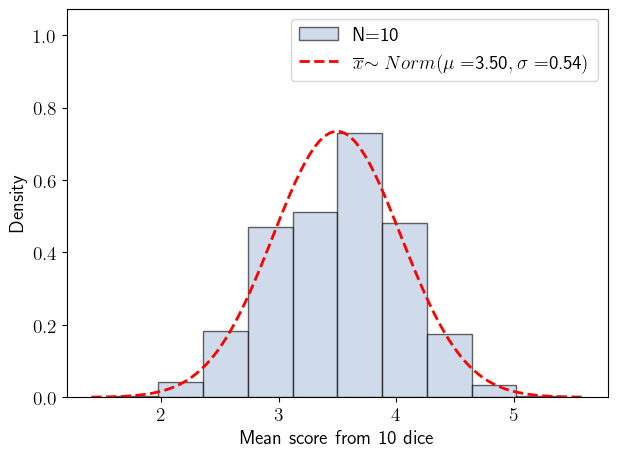
\includegraphics[scale=0.4]{CLT-uniform-N10-Z10000-meanandfit.png}}
\only<2>{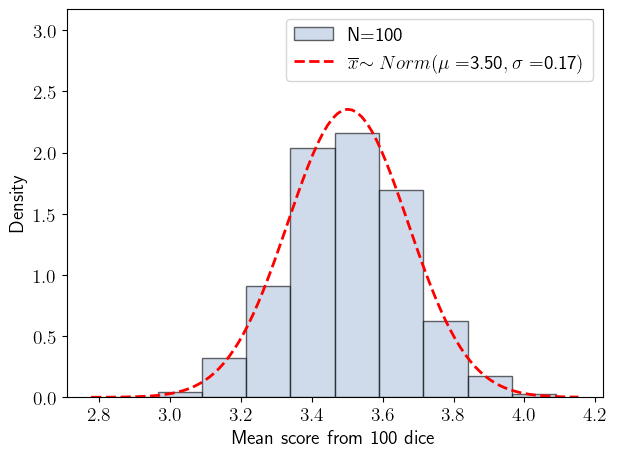
\includegraphics[scale=0.4]{CLT-uniform-N100-Z10000-meanandfit.png}}
\only<3>{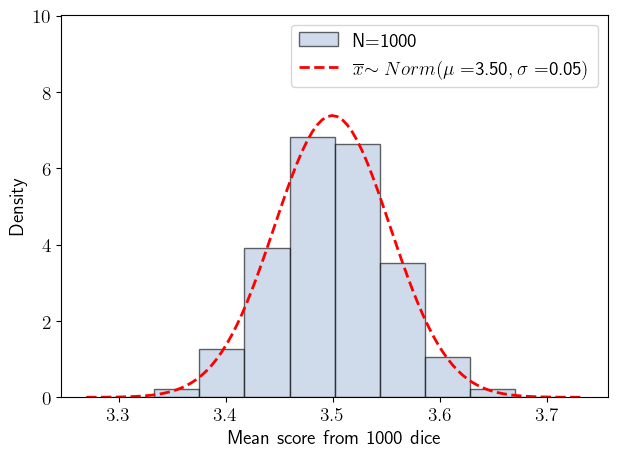
\includegraphics[scale=0.4]{CLT-uniform-N1000-Z10000-meanandfit.png}}
\only<4>{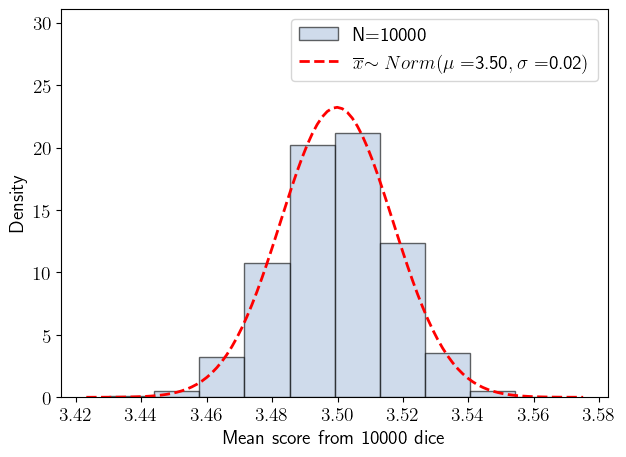
\includegraphics[scale=0.4]{CLT-uniform-N10000-Z10000-meanandfit.png}}
\only<5>{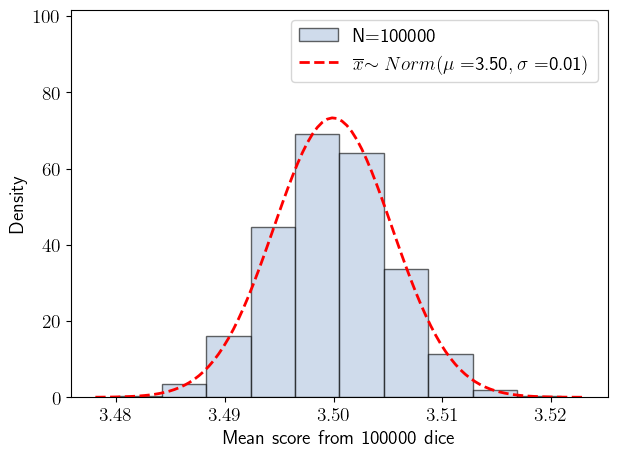
\includegraphics[scale=0.4]{CLT-uniform-N100000-Z10000-meanandfit.png}}
 \end{center}
 
 \end{frame}



\begin{frame}{The CLT: Standard Normal RV}
\footnotesize

Recall the Standard Normal RV: $Z =  \dfrac{X-\mu}{\sigma} \equiv  \dfrac{X-E[X] }{\sqrt{V[X]}}$. \\[1ex]

This is a particularly nice RV because $E[Z] = 0$ and $V[Z] = 1$ by definition, and it is a piece of cake to calculate probabilities with the Standard normal CDF (not analytically!)\\[1ex]

\texttt{\# default params for scipy.stats norm are loc=0, scale=1}\\[1ex]
$P(|Z| \leq \bbl{1}) = \rbl{68.27\%}$\; \; \texttt{norm.cdf(1)}\\[1ex]
$P(|Z| \leq \bbl{2}) = \rbl{95.45\%}$\; \; \texttt{norm.cdf(2)}\\[1ex]
$P(|Z| \leq \bbl{3}) = \rbl{99.73\%}$\; \; \texttt{norm.cdf(3)}\\[1ex]

\magt{CLT: we can use this cake-walk method to estimate probabilities for sums of means of RVs from any distribution.}
\end{frame}


\begin{frame}{The mean of $N$ RVs as a Standard Normal RV}
\footnotesize
$Z =  \dfrac{X-\mu}{\sigma} \equiv  \dfrac{X-E[X] }{\sqrt{V[X]}}$\;\; We will let $X\rightarrow \overline{X}$. \\[1ex]

Denominator: $\sqrt{V[\,\overline{X}\,]} = \sqrt{V[\,X\,] / N } =$ \ghl{$\sigma/\sqrt{N }$}\\[1ex]

\uncover<2->{ Numerator: $\overline{X} - E[\,\overline{X}\,] = $\ghl{$\frac{1}{N}\sum\limits_i^N X_i - E[\,\frac{1}{N}\sum\limits_i^N X_i\,] $}}\\[1ex]

\uncover<3>{ Letting $Y = \sum\limits_i^N X_i$, and noting $N/\sqrt{N} = \sqrt{N} $, we have:\\[1ex]
\begin{center}
\bhl{$Z_N = \dfrac{ Y -  E[Y] }{ \sqrt{N}\, \sigma}$}\\[1ex]
\end{center}
}
\end{frame}


\begin{frame}{Probabilities for sum or mean of RVs\; \small{\bhl{$Z_N = \dfrac{ Y -  E[Y] }{ \sqrt{N}\, \sigma}$} } }
\footnotesize
To calculate probabilities for our $Y=\sum\limits_i^N X_i$, we use $Z_N$:\\[1ex]

$P(\rbl{y_{low}} \leq Y \leq \bbl{y_{high}} ) = 
P\left( 
\rbl{ \dfrac{ y_{low} -  E[Y] }{ \sqrt{N}\, \sigma} }  
\leq\; 
\bhlm{Z_N}
\; \leq  
\bbl{\dfrac{ y_{high} -  E[Y] }{ \sqrt{N}\, \sigma} }
\right)$\\[3ex]

This looks a bit much, but is very easy to handle if we know $N$, $E[Y]$, and $\sigma$. See python example (just a few lines). \\[1ex]

Any measurement can be thought of as a Random Variable $X_i$.  The sum of IID\magt{*} $X_i$ is also a Random Variable $Y$. This will follow Norm(0,1) if the number of measurements of $X_i$ used to construct it is large enough.\\


\magt{*Particle Physicists and other cowboys have been known to bend the rule that $X_i$ must be IID with very pleasing results!}


\end{frame}





\section{Hypo}

\begin{frame}{Hypotheses}
\footnotesize

A \boo{Hypothesis}  is an educated guess at the explanation for some occurrence. It must be based on real observations and \textbf{it must be testable}.\\[1ex]

For example, if I collect some data (and I do not know the underlying PDF) I may observe that it looks like exponential decay when I plot it,  but it has some lumps and bumps, so something more interesting could possibly be going on... \\[1ex]

The \boo{Null Hypothesis} $H_0$ is the educated guess that the most obvious (boring?) explanation for the data is the correct one. For the example above, the Null Hypothesis could be that the data is indeed Expon($\lambda$).\\[1ex]

The  \boo{Alternative Hypothesis} $H_1$ is an alternative to $H_0$. For the example above, the Alternative Hypothesis would be that the lumps and bumps are exciting resonances that will win your research group a nobel prize and pay for a new espresso machine.\\[1ex]
\end{frame}


\begin{frame}{Bias}
\footnotesize

\begin{columns}
\begin{column}{0.6\textwidth}
My tangible excitement at the idea of an alternative hypothesis should raise a big red flag.\\[1ex]

Anyone who has done Harvard's excellent \href{https://implicit.harvard.edu/implicit/takeatest.html}{Unconscious Bias tests} will know that humans are hopeless at being unbiased, even when we aren't aware that we have a bias.\\[1ex]

This means that if we are going to do excellent science, and not just come up with whatever result means we get a new espresso machine, we have to remove any chance of introducing bias.\\[1ex]

One way of doing this is to set out very strict criteria for the null and alternate hypotheses before we look at our data.\\[1ex]

\end{column}

\begin{column}{0.4\textwidth}

\includegraphics[scale=0.2]{espresso}
\end{column}

\end{columns}
\end{frame}


\begin{frame}{Example of Null and Alternative Hypotheses}
\footnotesize
After waiting forever for the LHC to get going after some unfortunate stalls due to bad soldering and a ferret, we  started to see `Higgs-like' signs in 2011.\\

\begin{center}
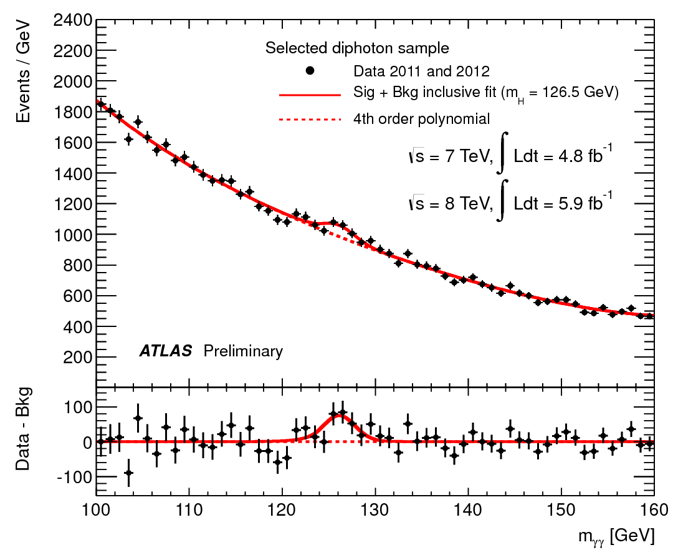
\includegraphics[scale=0.5]{higgs.png}
\end{center}
\end{frame}

\begin{frame}{Strict Criteria[1]: Define a Critical Region}
\footnotesize
A \boo{Critical Region} $W$ is a region of the Sample Space in which the probability of finding the data, given the Null Hypothesis, is very small. \\[1ex] 
The region $W$ can have any shape, making it suitable for tests involving multivariate data. The simplest possible definition of $W$ for univariate data would be to draw a vertical line (a `cut') and define $W$ as being on one side of it.\\[1ex]
A \boo{Positive Result} means that we have found our data $x$ in $W$, and so we \boo{reject the Null Hypothesis}.\\[1ex]
\bbl{One cannot prove a hypothesis. Hypotheses can only be rejected or not rejected.}\\[1ex]
In reality it is impossible to find a $W$ that is not consistent with both $H_0$ and $H_1$. If we could, we would not need to do any of this....

\end{frame}

\begin{frame}{Strict Criteria [2]: Significance Level}
\footnotesize
``Define a \boo{Critical Region} $W$. This is a region of the Sample Space in which the probability of finding the data, given the Null Hypothesis, is \bbl{very small}.'' \\[1ex] 
What does \bbl{very small} mean?\\[1ex]
A popular choice in the wide world (but not in my world) is to set a tolerance level of $5\%$. We define our region $W$ such that there is a $5\%$ or lower probability of finding the data in that region, given the null hypothesis $H_0$.\\[1ex]
This is called the \boo{Significance Level}, $\alpha$.\\[1ex]
\begin{center}
\bhl{$P(x\in W | H_0) \leq \alpha$}\\[1ex]
\end{center}
Once we when we have decided on $W$ and $\alpha$, we can look at (`unblind') our data.\\[1ex]

\end{frame}


\begin{frame}{Choosing a Critical Region is challenging}
\footnotesize
\begin{columns}
\begin{column}{0.5\textwidth}
\begin{center}
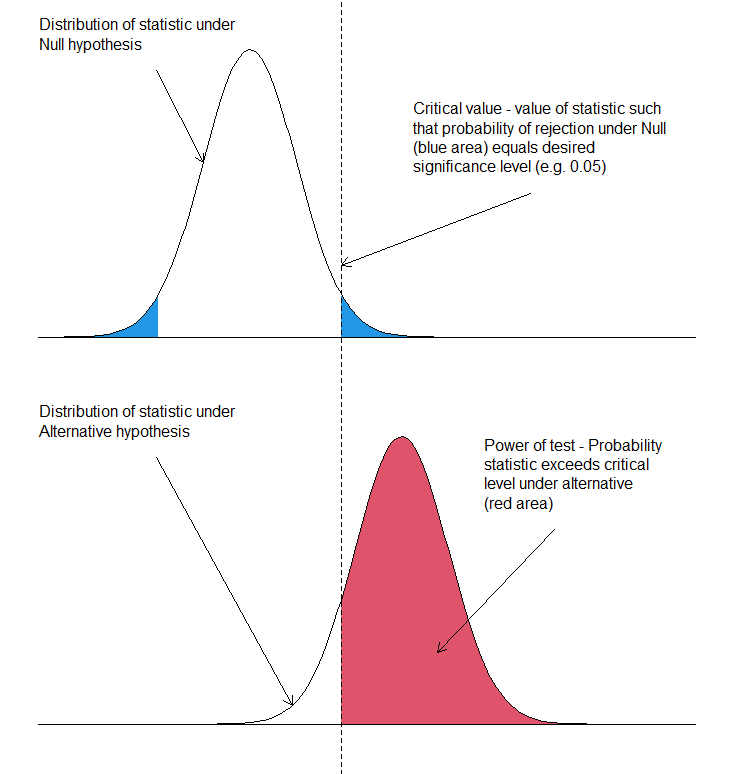
\includegraphics[scale=0.2]{PowerOfTest.png}
\tiny
\href{https://creativecommons.org/licenses/by/4.0}{Credit: Fangz CC BY 4.0}
\end{center}
\end{column}
\begin{column}{0.5\textwidth}
\bbl{Is purity or efficiency more important to you?} High purity means small $\alpha$ (small contamination) and lower power (you have cut out a lot of your sample). \\[2ex]
\bbl{Are you suffering from a small dataset?} If so, you will probably have to maximise power at the cost of purity.\\[2ex]
\rbl{Will your funding be withdrawn if you don't publish?} This is not a valid reason to make a scientific decision, but is shockingly common (see later). \\[1ex]
\end{column}
\end{columns}

\end{frame}








\begin{frame}{Limitations of the Statistical Test}
\footnotesize

\bbl{If we find our data satisfies our predefined statistical test $P(x\in W | H_0) \leq \alpha$}, then we have some responsibility to publish.
\begin{itemize}
\item With a Significance Level of $\alpha= 5\%$, this would give me major heeby jeebies.
\item The statistical test for rejecting $H_0$ has a \boo{False Positive} rate of up to 5\%, which to me seems enormous. A one in twenty chance that this is...wrong. 
\item This is called a \boo{Type 1 Error}.
\end{itemize}
\vspace{0.5cm}

\bbl{If we find our data fails our predefined statistical test}, then we have no reason to reject $H_0$.
\begin{itemize}
\item This does not mean $H_0$ is correct; a hypothesis cannot be shown to be correct. It could be that we just got unlucky - the data ended up in some other critical region that we did not choose for our predefined statistical test. 
\item This is a \boo{False Negative} or \boo{Type 2 Error}
\end{itemize}

\end{frame}

\begin{frame}{The Confusion Matrix \only<4-5>{\magt{Type 2 Error} }  \only<8-9>{\boo{Type 1 Error!} } }

\only<1>{
\begin{center}
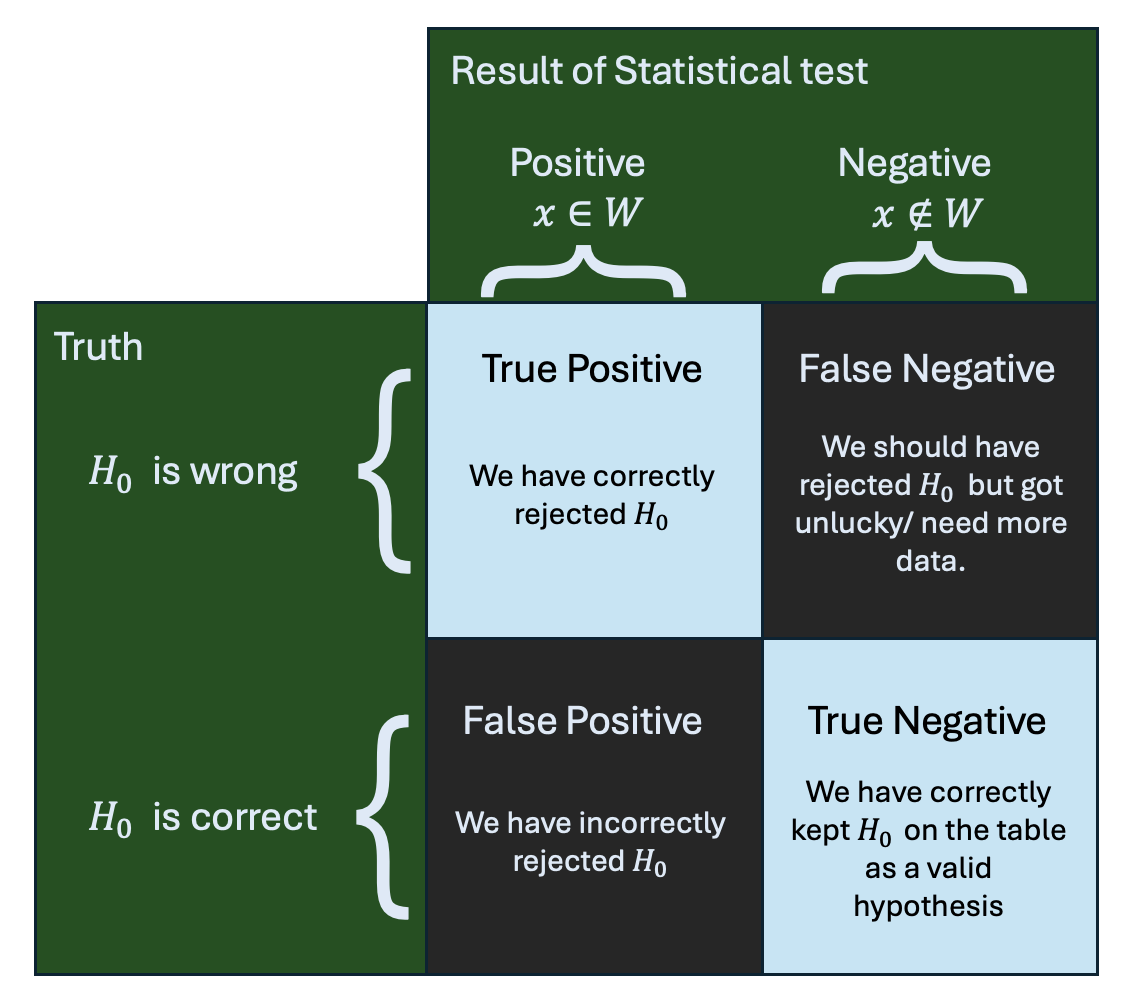
\includegraphics[scale=0.37]{conm.png}
\end{center}
}
\only<2>{
\begin{center}
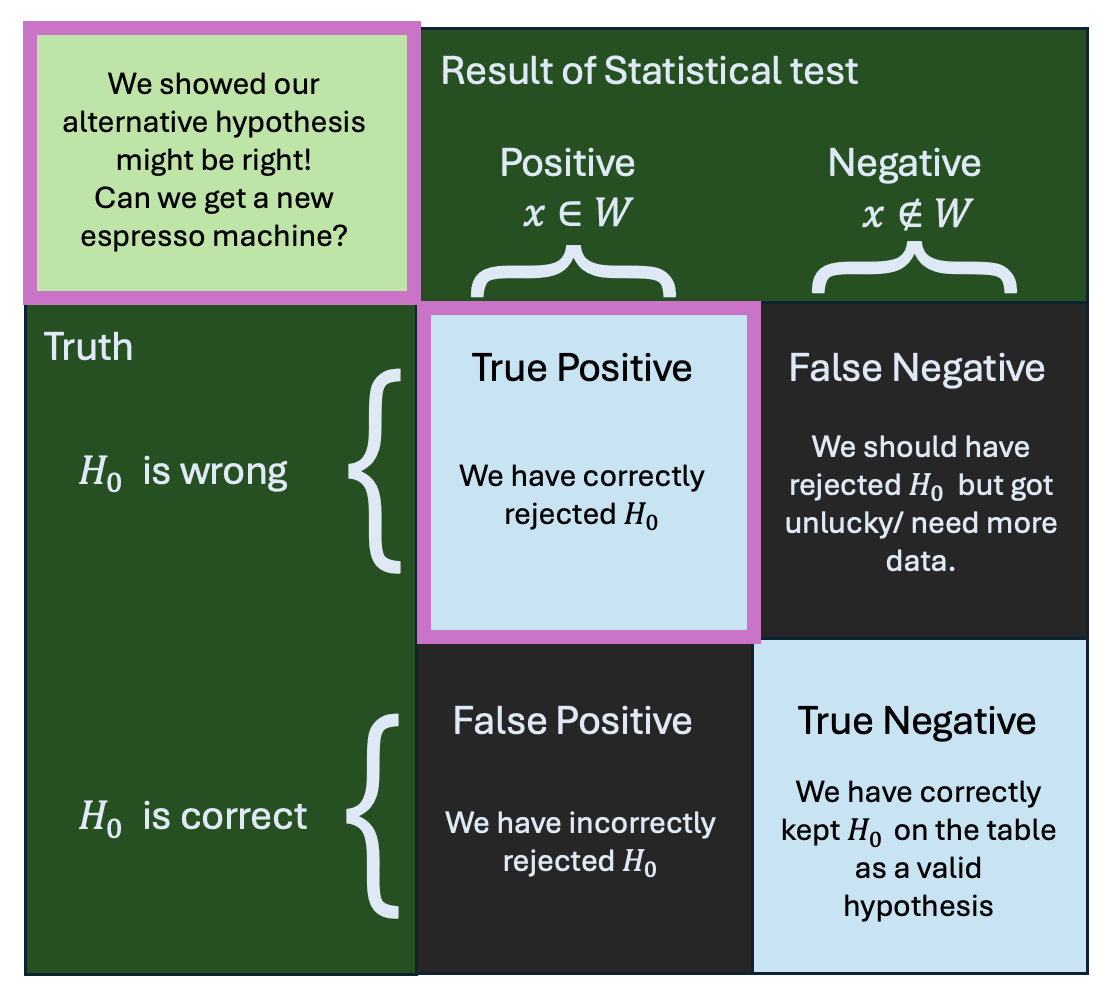
\includegraphics[scale=0.37]{conm1.png}
\end{center}
}
\only<3>{
\begin{center}
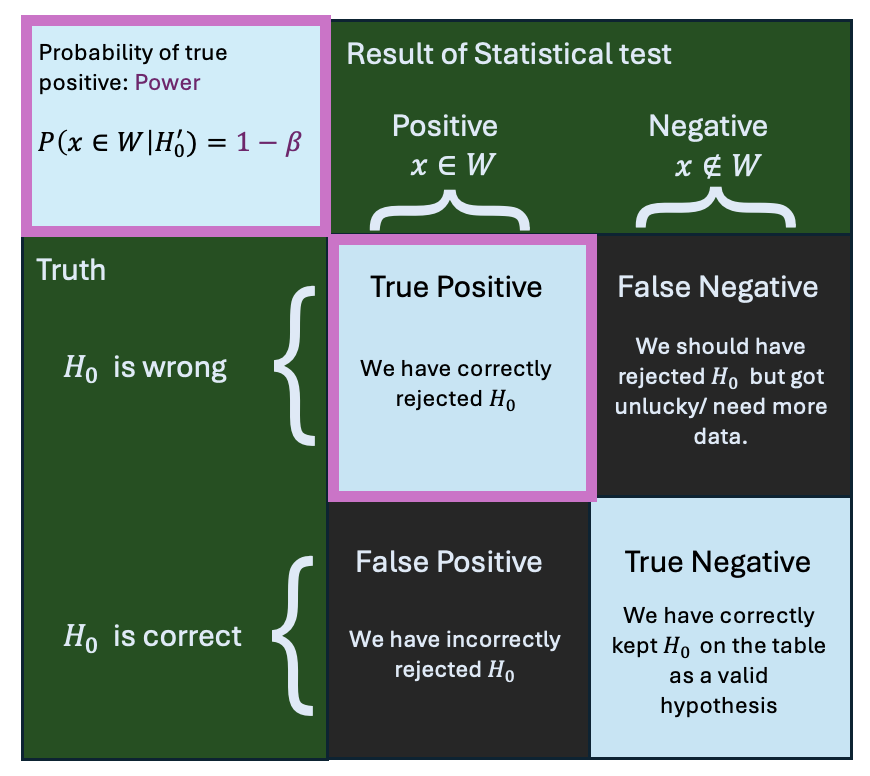
\includegraphics[scale=0.47]{conm1b.png}
\end{center}
}
\only<4>{
\begin{center}
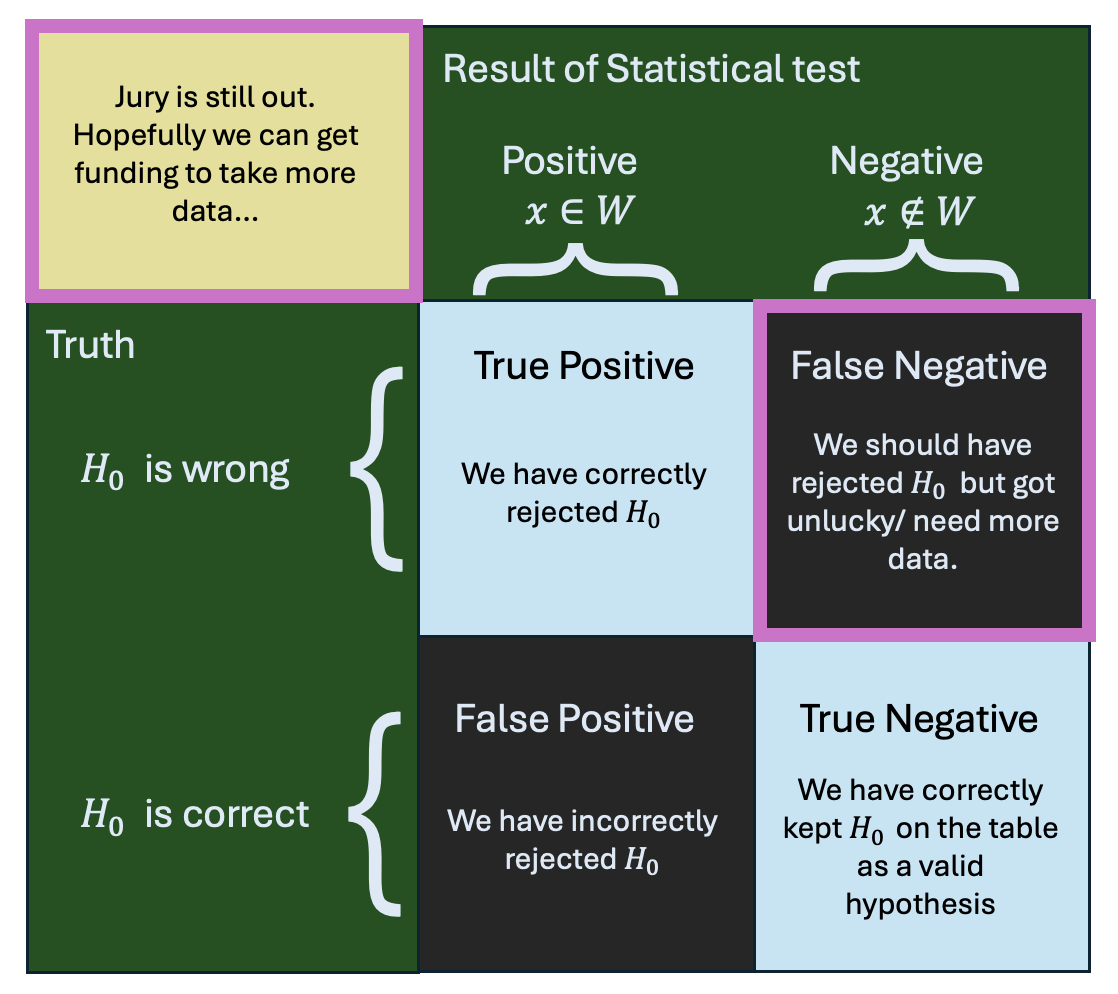
\includegraphics[scale=0.37]{conm2.png}
\end{center}
}
\only<5>{
\begin{center}
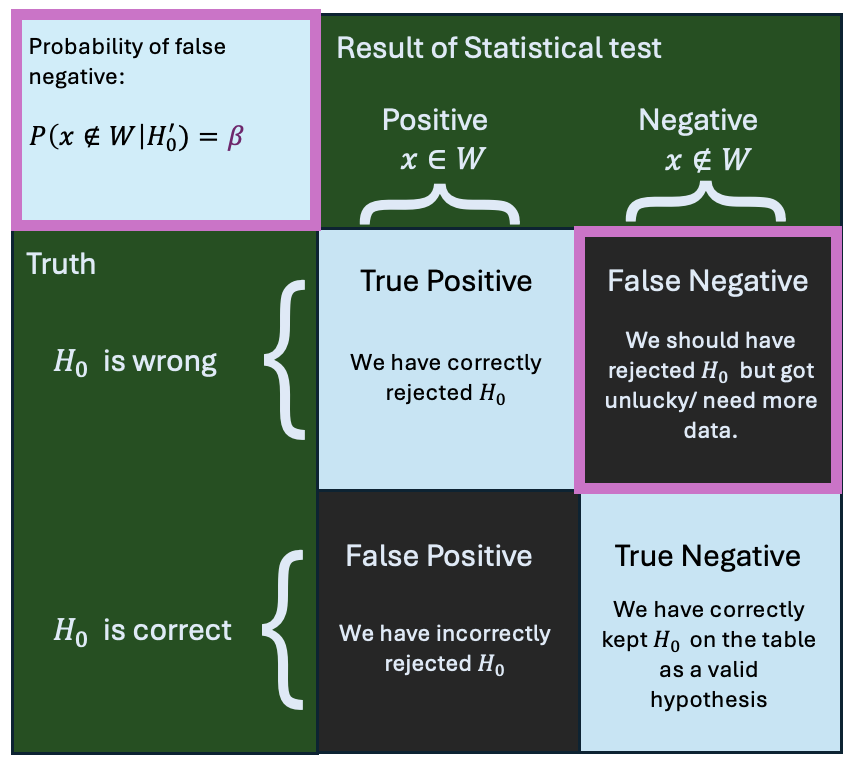
\includegraphics[scale=0.47]{conm2b.png}
\end{center}
}
\only<6>{
\begin{center}
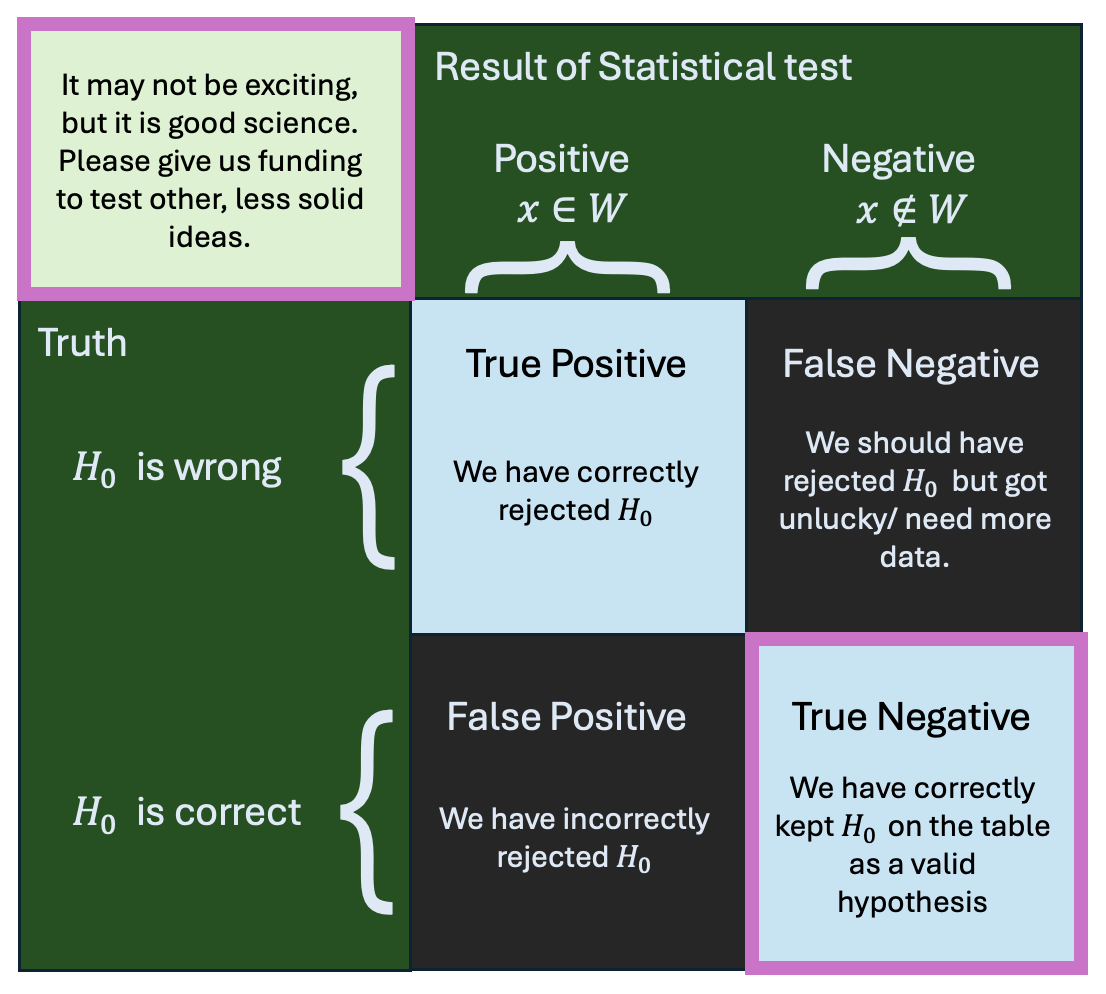
\includegraphics[scale=0.37]{conm3.png}
\end{center}
}
\only<7>{
\begin{center}
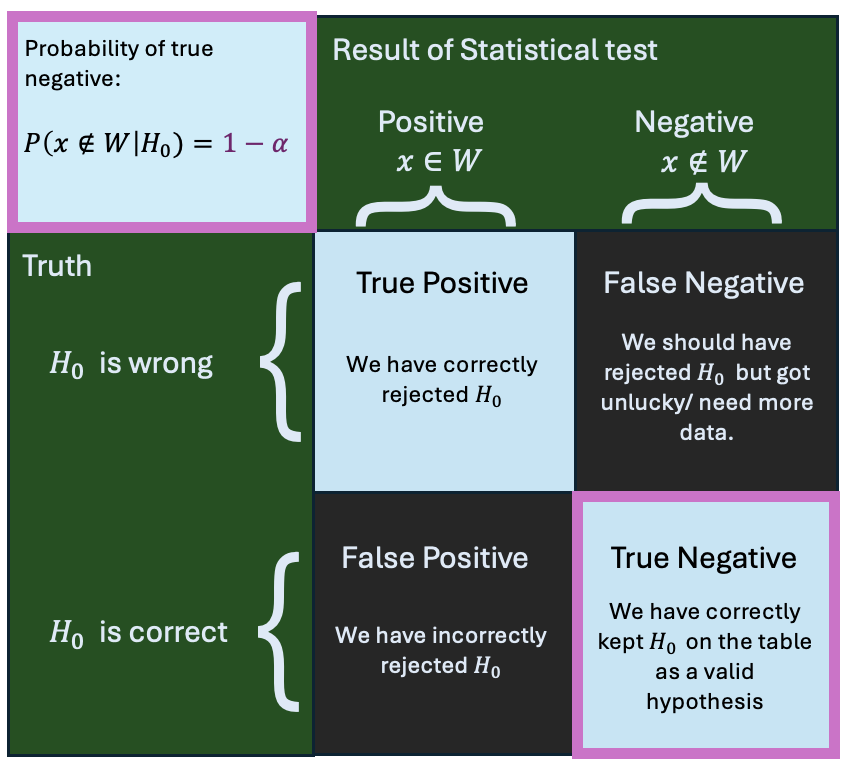
\includegraphics[scale=0.47]{conm3b.png}
\end{center}
}
\only<8>{
\begin{center}
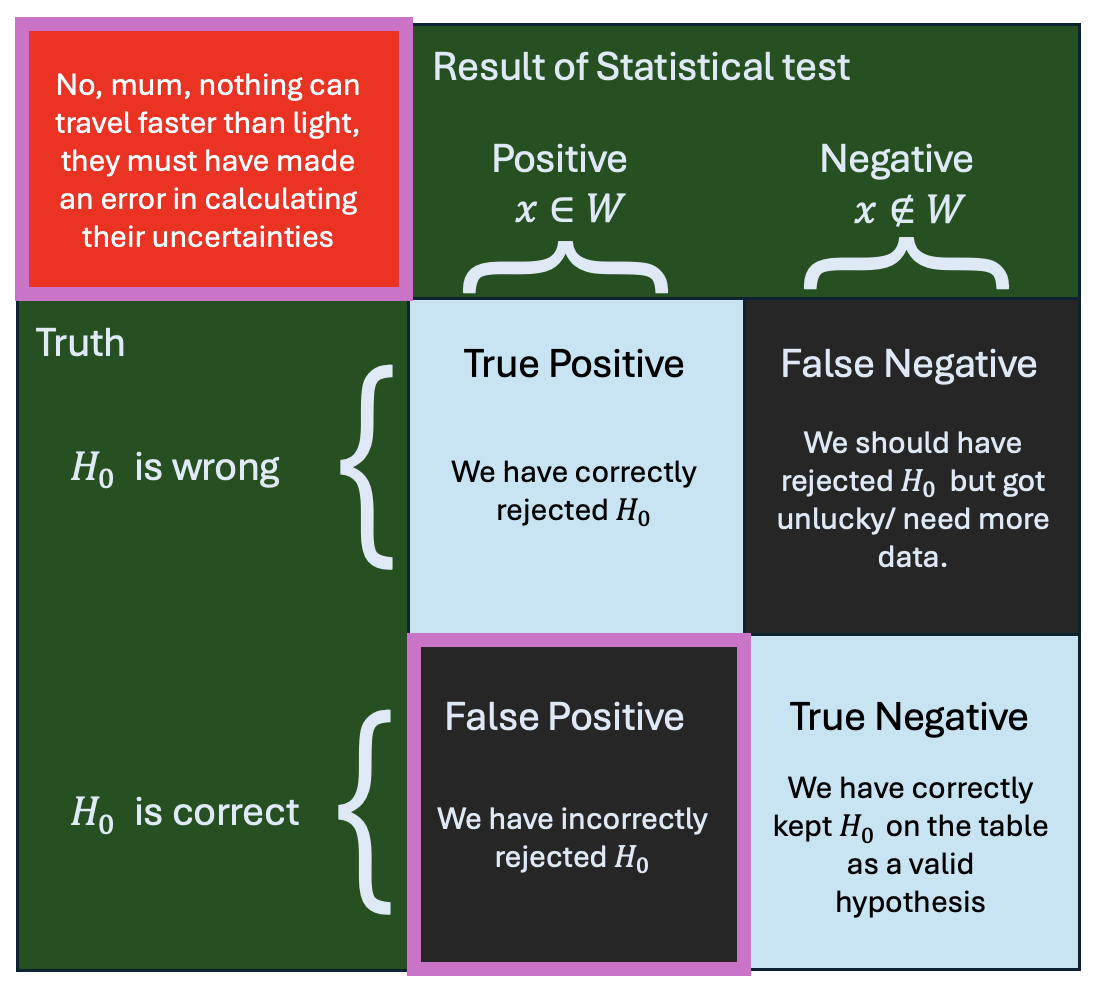
\includegraphics[scale=0.37]{conm4.png}
\end{center}
}
\only<9>{
\begin{center}
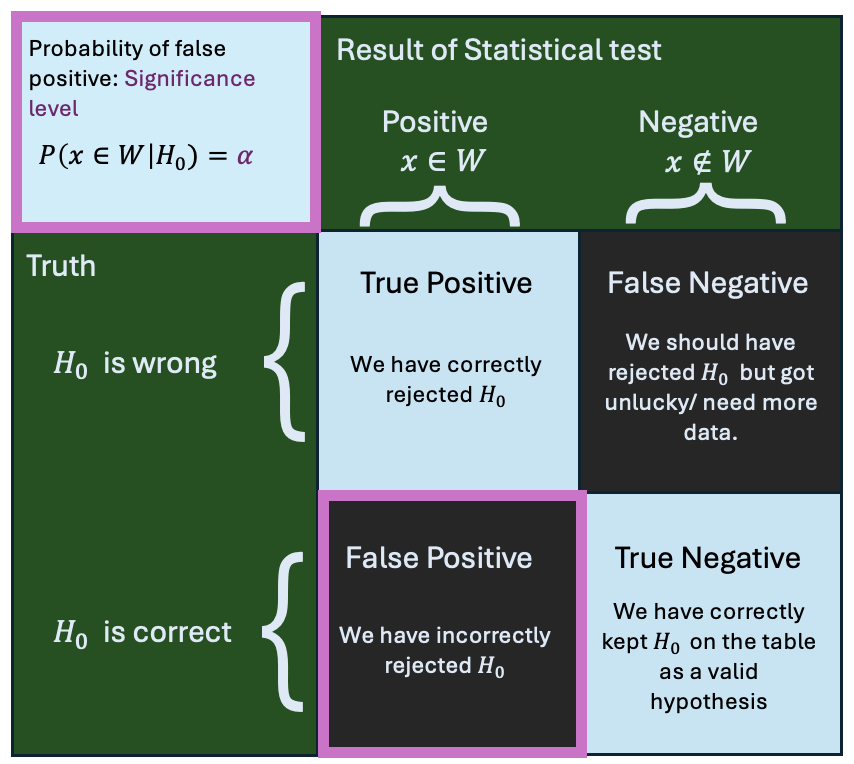
\includegraphics[scale=0.47]{conm4b.png}
\end{center}
}

\end{frame}




\section{P-val}





\begin{frame}{p-values and z-values}
\footnotesize
The Significance of a measurement is expressed in terms of either a p-value or z-value, both of which are calculated from the data.\\[1ex]
\begin{center}
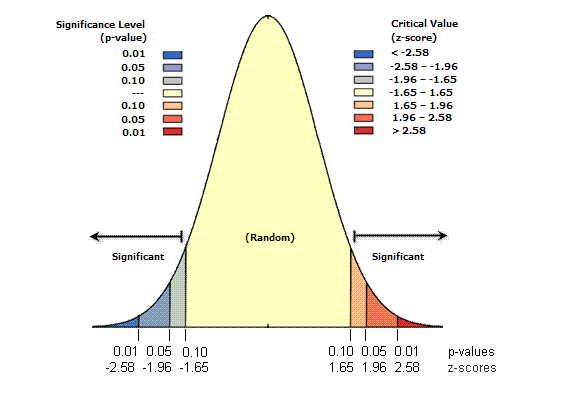
\includegraphics[scale=0.82]{pz.png}\tiny
\href{https://pro.arcgis.com/en/pro-app/latest/tool-reference/spatial-statistics/what-is-a-z-score-what-is-a-p-value.htm}{Credit: ArcGIS Pro 3.5}
\end{center}

\end{frame}






\begin{frame}{p-values and Z-values}
\footnotesize

We know the z-value already: $z=\dfrac{x-\mu}{\sigma}$. This tells us the deviation of our data $x$ from the expected value $\mu$ in units of `number standard deviations from the mean' or $n\sigma$.\\[1ex]

For example there is a $68\%$ probability of observing normally distributed data within the $\pm1\sigma$ region of the standard normal distribution.\\[1ex]

The Standard Normal PDF: $f_Z(x-\mu;\sigma) = \dfrac{1}{\sigma \sqrt{2\pi}} exp\left[-\dfrac{z^2}{2}\right]$ \\[1ex]

The Standard Normal CDF: $F_Z(x-\mu;\sigma) = \dfrac{1}{ \sqrt{2\pi}}\, \int\limits_{-\infty}^{z}\, exp\left[-\dfrac{z^2}{2}\right] dz $\\[1ex]


\end{frame}




\begin{frame}{p-values and z-values}
\footnotesize
The Standard Normal CDF: $F_Z(x-\mu;\sigma) = \dfrac{1}{ \sqrt{2\pi}}\, \int\limits_{-\infty}^{z}\, exp\left[-\dfrac{z^2}{2}\right] dz $\\[1ex]

We can't solve this integral analytically, so we look up the probabilities (or use python).\\[1ex]

$P(|Z| \leq \bbl{1}) = \rbl{68.27\%}$, \bbl{z-value is $1\sigma$}, \rbl{p-value is $(1 - 68.27\%) = 0.3173 $}\\[1ex]
$P(|Z| \leq \bbl{2}) = \rbl{95.45\%}$, \bbl{z-value is $2\sigma$}, \rbl{p-value is $(1 - 95.45\%) = 0.0455 $}\\[1ex]
$P(|Z| \leq \bbl{3}) = \rbl{99.73\%}$, \bbl{z-value is $3\sigma$}, \rbl{p-value is $(1 - 99.73\%) = 0.0027 $}\\[1ex]

The p-value is the area under a portion of a tail of the standard normal distribution, where the normal distribution represents the null hypothesis. A very small p-value (high z-value) means it is very unlikely that we would find the data there, given the null hypothesis.
\end{frame}



\begin{frame}{Poor Decision Making (medical publications)}
\footnotesize
This plot shows the distribution of z-values (significance levels) in published medical journals over the last fifty years.
\begin{columns}
\begin{column}{0.6\textwidth}
\begin{center}
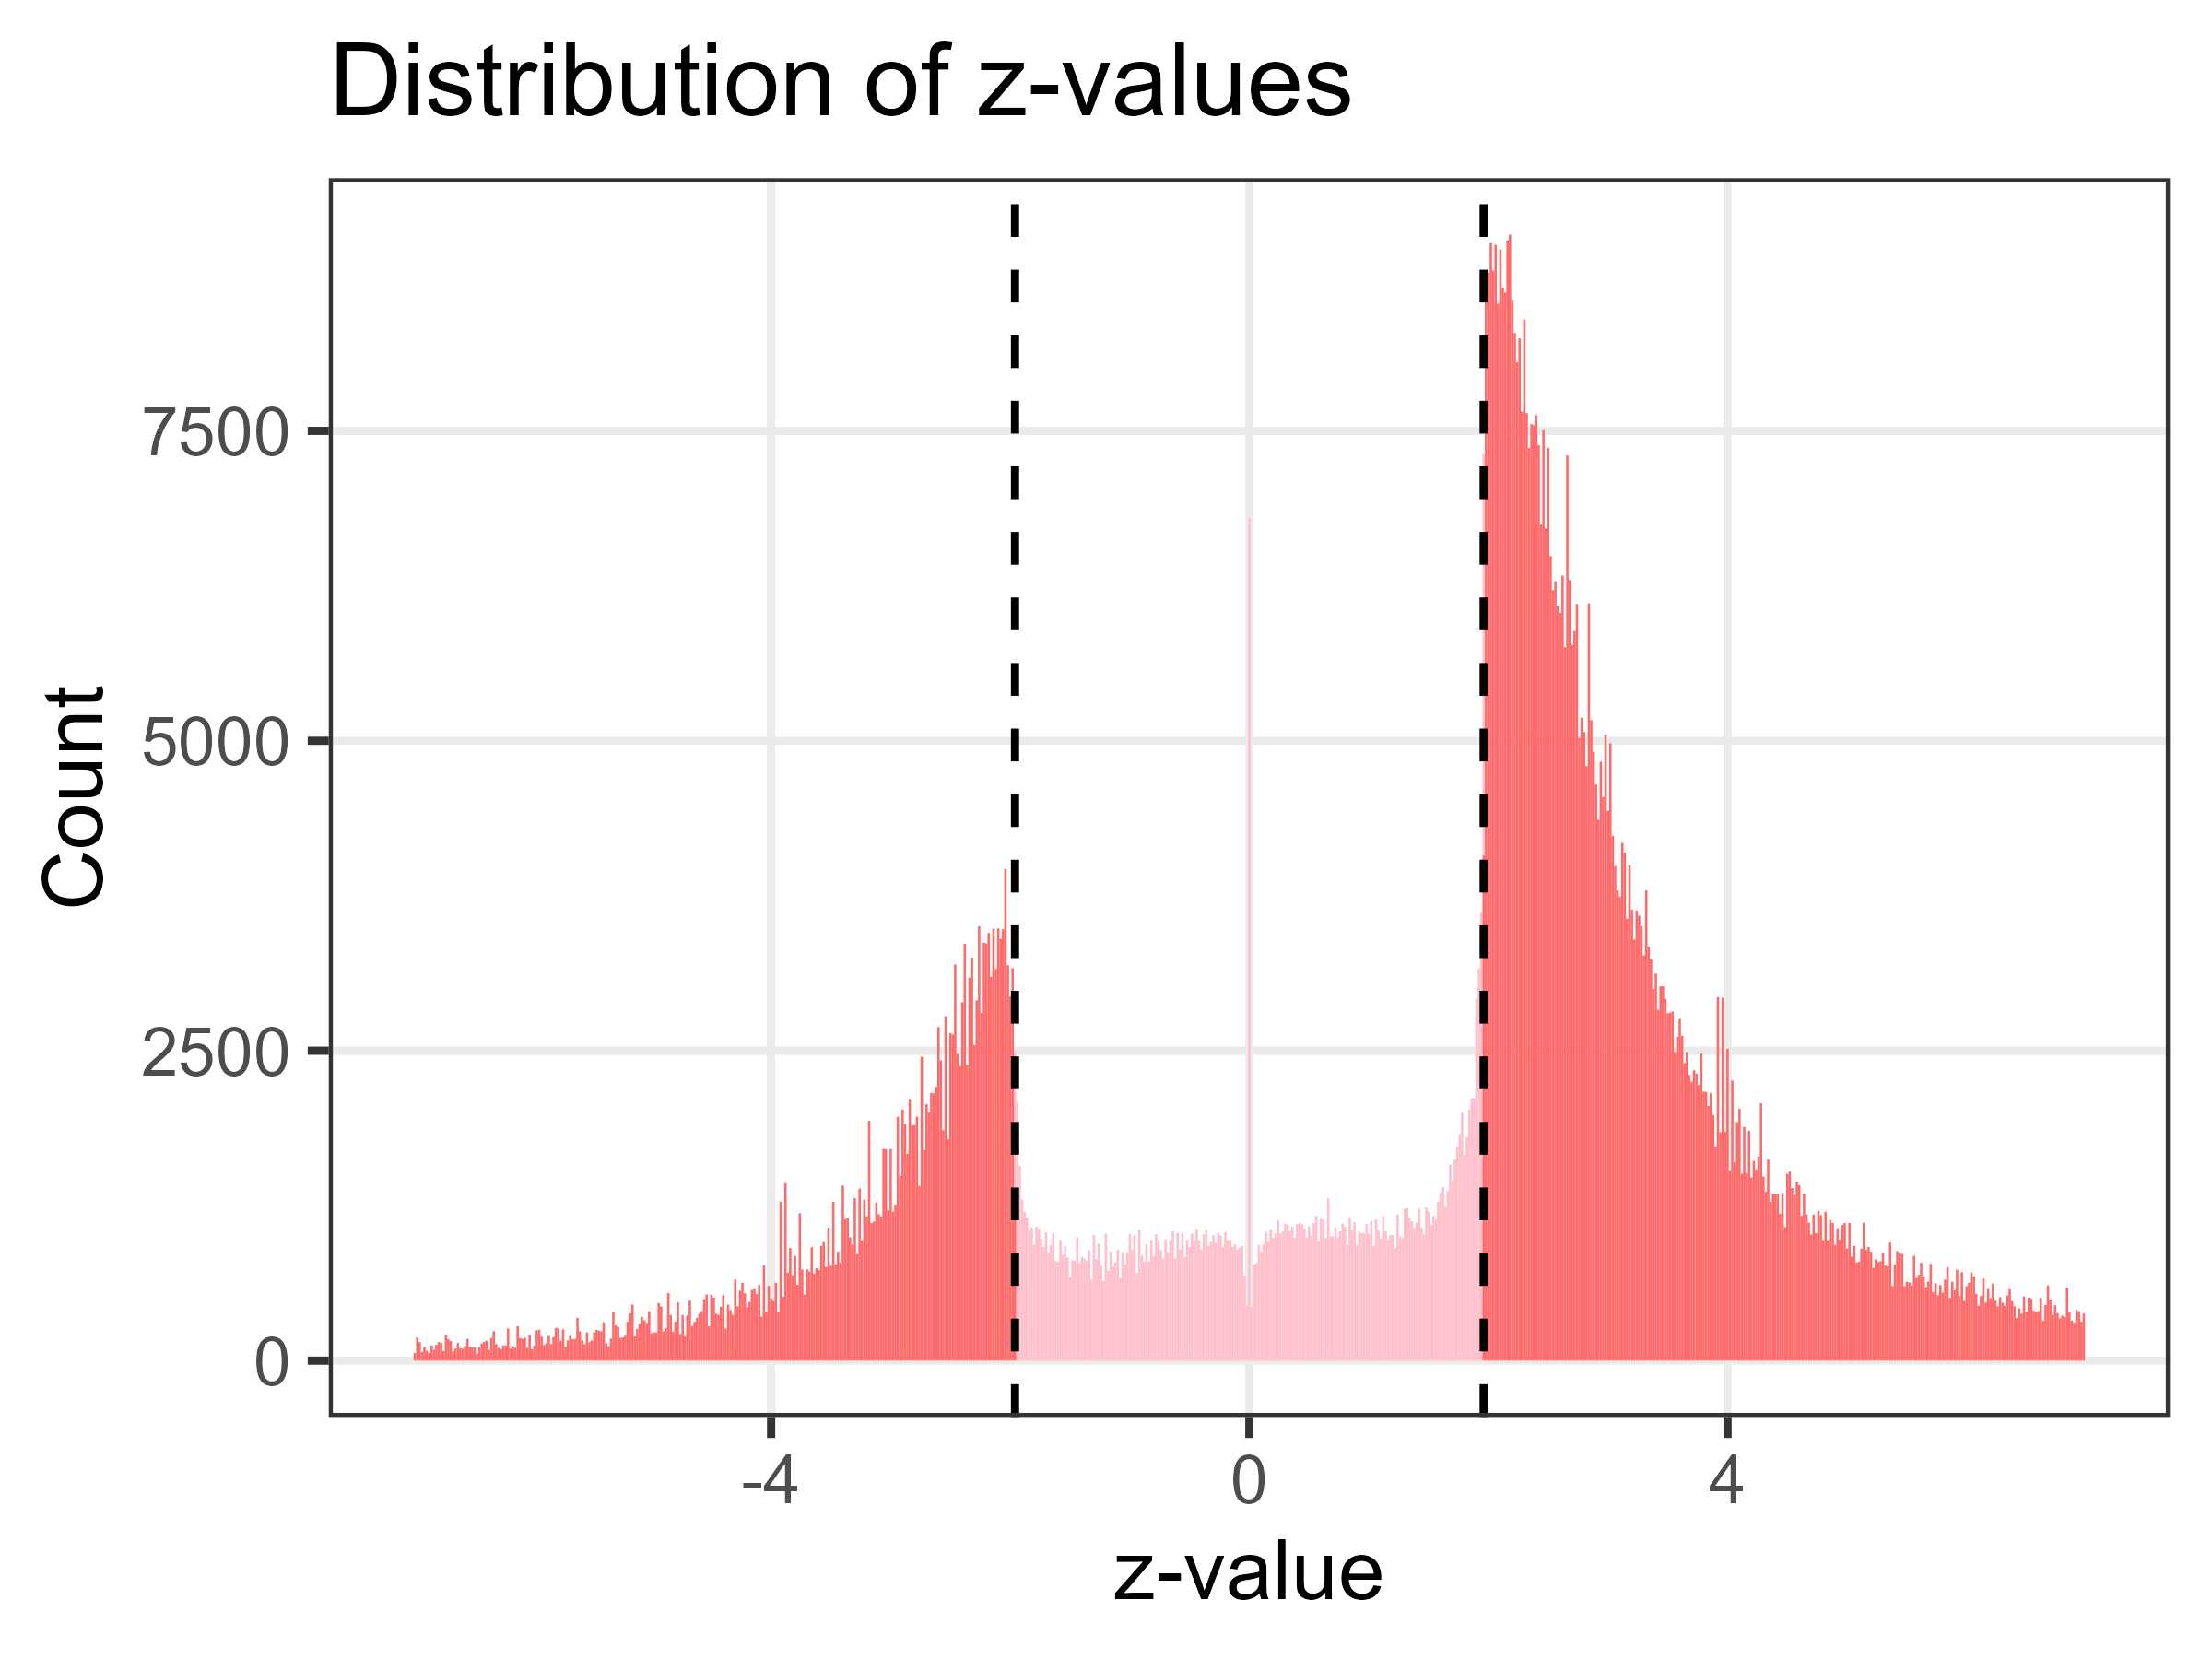
\includegraphics[scale=0.63]{Z_plot.png}
\tiny
\href{https://medianwatch.netlify.app/post/z_values/}{Credit: Erik Van Zwet, Adrian Barnett}
\end{center}
\end{column}
\begin{column}{0.4\textwidth}
The data bear resemblance to a normal distribution (good) but most of the middle section (p-values greater than $5\%$) has been blown away.\\[1ex]
This indicates \boo{very bad science} (manipulating the tests/results) exacerbated by journals tending to reject work that fails to reject the null hypothesis, and funding relying on publications.
\end{column}
\end{columns}
\end{frame}



\begin{frame}{Confidence Levels, Limits, Intervals}
\footnotesize
\begin{itemize}
\item A \boo{Confidence Level} often used is $95\%$, which corresponds to a p-value of $5\%$ (the favourite of dodgy medical researchers) and a z-value of $1.644\sigma$.
\item The $95\%$ \boo{Confidence Interval} includes all values within $1.644\sigma$ of the mean of a normal distribution.
\item The \boo{Confidence Limits} in this case are $\mu+1.644\sigma$ and $\mu-1.644\sigma$ 
\end{itemize}
\vspace{0.5cm}

\textbf{A CL of $95\%$ means is that if we were to repeat the experiment 100 times, we would expect the true mean to lie in the Confidence Interval 95 times.}\\[1ex]

\footnotesize
$P(|Z| \leq \bbl{1.644}) = \rbl{95\%}$, \bbl{z-value is $1.644\sigma$}, \rbl{p-value is $(1 - 95\%) = 0.05 $}\\[1ex]

\texttt{p-value = 1-norm.cdf(z-value);\;\;\; z-value = norm.ppf(1 - p-value)}


\end{frame}




\begin{frame}{Thanks For Your Time}
\center
\Huge
Fin.
\end{frame}






\end{document}
 